\documentclass[12pt]{kiarticle} % You can learn about my document class "kiarticle" and install it to your device by following the link: https://github.com/Kiarendil/toolkitex
\graphicspath{{pictures/}}
\DeclareGraphicsExtensions{.pdf,.png,.jpg,.eps}
%%%
\pagestyle{fancy}
\fancyhf{}
%\renewcommand{\headrulewidth}{ 0.1mm }
\renewcommand{\footrulewidth}{ .0em }
\fancyfoot[C]{\texttt{\textemdash~\thepage~\textemdash}}
\fancyhead[L]{Лабораторная работа № 3.6.1 \hfil}
\fancyhead[R]{\hfil Иванов Кирилл, 625 группа }
\usepackage{multirow} % Слияние строк в таблице
\newcommand
{\un}[1]
{\ensuremath{\text{#1}}}
\newcommand{\eds}{\ensuremath{ \mathscr{E}}}
\usepackage{tikz}
%%% Работа с таблицами
\usepackage{array,tabularx,tabulary,booktabs} % Дополнительная работа с таблицами
\usepackage{longtable}  % Длинные таблицы
\usepackage{multirow} % Слияние строк в таблице

\begin{document}
	
	\begin{titlepage}
	\begin{center}
		\large 	Московский физико-технический институт \\
		(государственный университет) \\
		Факультет общей и прикладной физики \\
		\vspace{0.2cm}
		
		\vspace{4.5cm}
		Лабораторная работа № 3.6.1 \\ \vspace{0.2cm}
		\large (Общая физика: электричество и магнетизм) \\ \vspace{0.2cm}
		\LARGE \textbf{Спектральный анализ электрических сигналов}
	\end{center}
	\vspace{2.3cm} \large
	
	\begin{center}
		Работу выполнил: \\
		Иванов Кирилл,
		625 группа
		\vspace{10mm}		
		
	\end{center}
	
	\begin{center} \vspace{60mm}
		г. Долгопрудный \\
		2017 год
	\end{center}
\end{titlepage}
	
	\paragraph*{Цель работы:} изучение спектрального состава периодических электрических сигналов.
	
	\paragraph*{Оборудование:} анализатор спектра, генератор прямоугольных импульсов, генератор сигналов специальной формы, осциллограф.
	
	\section{Теоретическая введение}
	
	Представление периодического сигнала в виде суммы гармонических сигналов называется разложением в ряд Фурье.
	
	Пусть заданная функция $f(t)$ периодически повторяется с частотой $\Omega_{1}=\dfrac{2\pi}{T},$ где $T$ - период повторения. Ее разложение в ряд Фурье имеет вид
	
	$$ f(t)=\dfrac{a_{0}}{2}+ \sum\limits_{n=1}^\infty [a_{n}\cos(n \Omega_{1}t)+b_{n}\sin(n \Omega_{1} t) ]$$
	
	Здесь $\dfrac{a_{0}}{2}$ - среднее значение функции $f(t)$,
	
	$$ a_{n}=\dfrac{2}{T}\int\limits_{t_{1}}^{t_{1}+T}f(t)\cos(n \Omega_{1} t)dt, $$
	
	$$ b_{n}=\dfrac{2}{T}\int\limits_{t_{1}}^{t_{1}+T}f(t)\sin(n \Omega_{1} t)dt. $$
	
	
	Рассмотрим периодические функции, которые исследуются в нашей
	работе.
	
	\begin{enumerate}
		
	\item 	\textbf{Периодическая последовательность прямоугольных импульсов} (рис. 1) с амплитудой $V_{0}$, длительностью $\tau$, частотой повторения $\Omega_{1}=\dfrac{2\pi}{T},$ где $T$ - период повторения импульсов. Найдем коэффициенты разложения ряда Фурье:
	
	$$\dfrac{a_{0}}{2}=V_{0}\dfrac{\tau}{T},$$
	
	$$a_{n}=\dfrac{2}{T}\int\limits_{-\frac{\tau}{2}}^{\frac{\tau}{2}}V_{0}\cos(n \Omega_{1} t)dt=2V_{0}\dfrac{\tau}{T}\dfrac{\sin(n \Omega_{1} \frac{\tau}{2})}{n\Omega_{1}\frac{\tau}{2}} \sim \dfrac{\sin x}{x}.$$
	
	Поскольку наша функция четная, все коэффициенты синусоидальных гармоник $b_{n}=0$. Спектр $a_{n}$ последовательности прямоугольных импульсов представлен на рис. 2 (изображен случай, когда $T$ кратно $\tau$).
		
		
		\begin{figure}[h]
			\begin{minipage}[h]{0.5\linewidth}
				\center{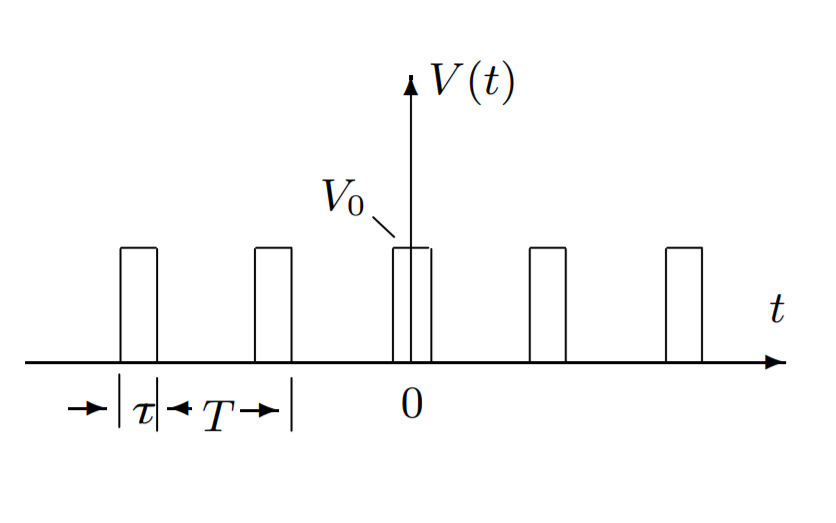
\includegraphics[width=0.9\linewidth]{sp1.png}}
				\caption{Прямоугольные импульсы}
			\end{minipage}
			\begin{minipage}[h]{0.5\linewidth}
				\center{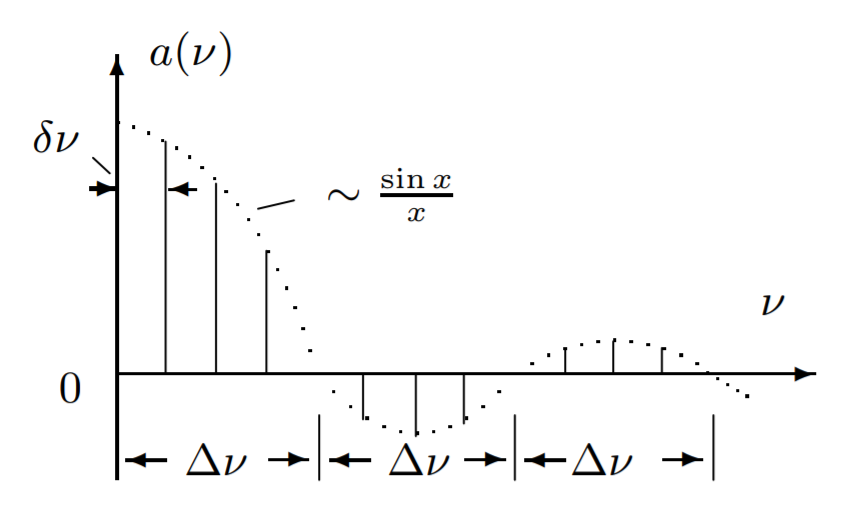
\includegraphics[width=0.9\linewidth]{sp2.png}}
				\caption{Спектр последовательности прямоугольных импульсов}
			\end{minipage}
		\end{figure}
	
	Назовем \textit{шириной спектра} $\Delta \omega$ расстояние от главного максимума ($\omega =0$) до первого нуля огибающей, возникающего при $n=\dfrac{2\pi}{\tau \Omega_{1}}$. При этом 

	$$\Delta \omega \tau \backsimeq 2 \pi $$
	
	 или 
	
\begin{equation}\label{neopr}
	\Delta \nu \Delta t \backsimeq 1
\end{equation}
		
	Полученное соотношение взаимной связи интервалов $\Delta \nu$ и $\Delta t$ является
	частным случаем соотношения неопределенности в квантовой механике.
	
	\item \textbf{Периодическая последовательность цугов} гармонического колебания $V_{0}\cos(\omega_{0}t)$ с длительностью цуга $\tau$ и периодом повторения $T$ (рис. 3).
	
	Функция $f(t)$ снова является четной относительно $t=0$. Коэффициент при $n$-й гармонике равен
	
	$$a_{n}=\dfrac{2}{T}\int\limits_{-\frac{\tau}{2}}^{\frac{\tau}{2}}V_{0}\cos(\omega_{0}t)\cos(n \Omega_{1} t)dt=V_{0}\dfrac{\tau}{T} \bigg(\dfrac{\sin[(\omega_{0}-n\Omega_{1})\frac{\tau}{2}]}{(\omega_{0}-n\Omega_{1})\frac{\tau}{2}}+\dfrac{\sin[(\omega_{0}+n\Omega_{1})\frac{\tau}{2}]}{(\omega_{0}+n\Omega_{1})\frac{\tau}{2}} \bigg)$$ 
	
	Зависимость для случая, когда $\frac{T}{\tau}$ равно целому числу, представлена на рис. 4. Сравнивая спектр последовательности прямоугольных импульсов и цугов мы видим, что они аналогичны, но их максимумы сдвинуты по частоте на величину $\omega_{0}$.
	
	\begin{figure}[h]
		\begin{minipage}[h]{0.5\linewidth}
			\center{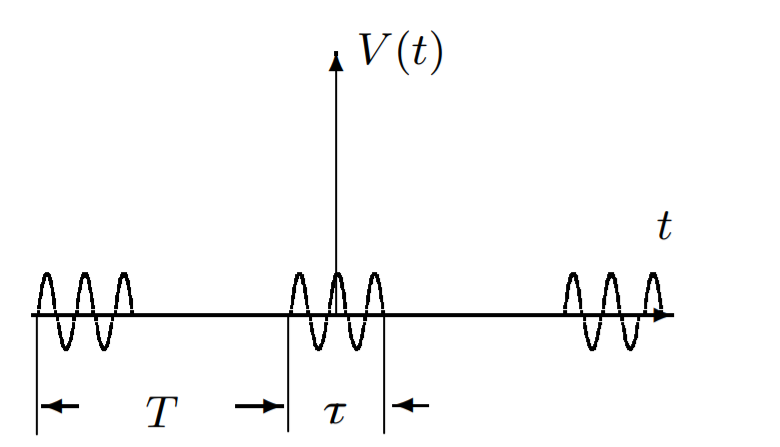
\includegraphics[width=0.9\linewidth]{sp3.png}}
			\caption{Последовательность цугов}
		\end{minipage}
		\begin{minipage}[h]{0.5\linewidth}
			\center{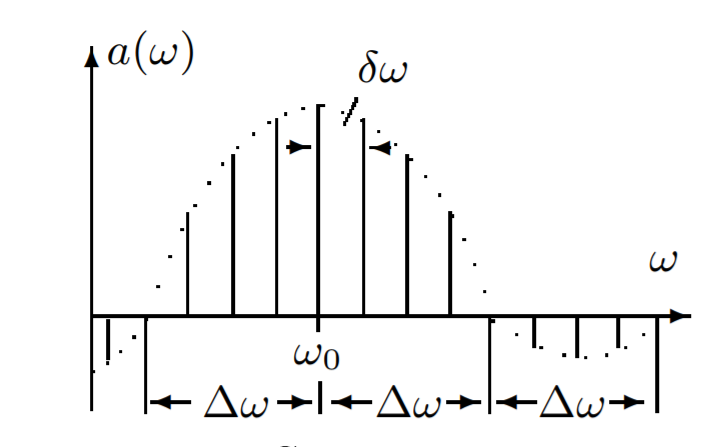
\includegraphics[width=0.9\linewidth]{sp4.png}}
			\caption{Спектр последовательности цугов}
		\end{minipage}
	\end{figure}

	\item \textbf{Амплитудно-модулированные колебания.} Рассмотрим гармонические колебания высокой частоты $\omega_{0}$ , амплитуда которых медленно меняется по гармоническому закону с частотой $\Omega$ ($\Omega \ll \omega_{0})$) (рис. 5):
	
	$$f(t)=A_{0}[1+m\cos\Omega t]\cos \omega_{0}t.$$
	
	Коэффициент $m$ называют \textbf{глубиной модуляции}. При $m<1$ амплитуда колебаний меняется от минимальной $A_{min}=A_{0}(1-m)$ до максимальной $A_{max}=A_{0}(1+m).$ Глубина модуляции может быть представлена в виде
	
\begin{equation}\label{m}
	 m=\dfrac{A_{max}-A_{min}}{A_{max}+A_{min}}
\end{equation}
	
	Простым тригонометрическим преобразованием можно найти спектр амплитудно - модулированных колебаний:
	\\
\begin{equation}\label{a}
	f(t)=A_{0}\cos(\omega_{0} t)+\dfrac{A_{0}m}{2}\cos(\omega_{0}+\Omega)t+\dfrac{A_{0}m}{2}\cos(\omega_{0}-\Omega)t.
\end{equation}
		
		\begin{figure}[h]
			\begin{minipage}[h]{0.5\linewidth}
				\center{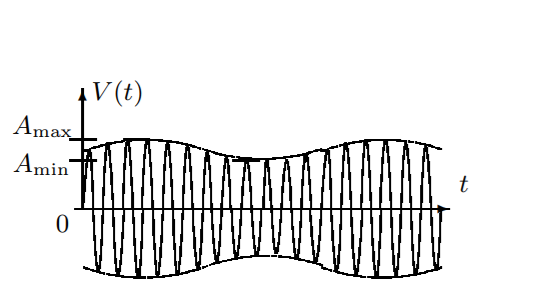
\includegraphics[width=0.9\linewidth]{sp5.png}}
				\caption{Модулированные гармонические колебания}
			\end{minipage}
			\begin{minipage}[h]{0.5\linewidth}
				\center{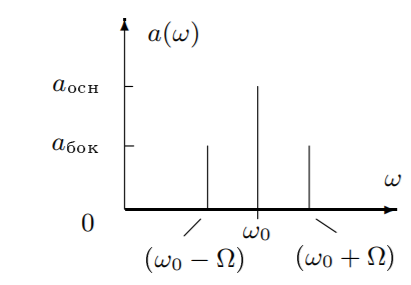
\includegraphics[width=0.9\linewidth]{sp6.png}}
				\caption{Спектр модулированных гармонических колебаний}
			\end{minipage}
		\end{figure}
		
		Спектр таких колебаний содержит три составляющих  основную
		компоненту и две боковых (рис. 6). Первое слагаемое в правой части представляет собой исходное немодулированное колебание
		с основной (несущей) частотой $\omega_{0}$ и амплитудой $a_{осн} = A_{0}$ . Второе и третье слагаемые соответствуют новым гармоническим колебаниям с частотами $\omega_{0} + \Omega$ и $\omega_{0} - \Omega$. Амплитуды этих двух колебаний одинаковы и составляют $\dfrac{m}{2}$ от амплитуды немодулированного колебания:
		$a_{бок} = \dfrac{A_{0}m}{2}$. Начальные фазы всех трех колебаний одинаковы.
	\end{enumerate}

	\section{Экспериментальные установки}
	
	\begin{enumerate}
		
		\item \textbf{Экспериментальная установка А} для исследования спектра периодической последовательности прямоугольных импульсов представлена на рис. 7. Сигнал с выхода генератора прямоугольных импульсов Г5-54 подается на
		вход анализатора спектра и одновременно  на вход Y осциллографа. С генератора импульсов на осциллограф подается также сигнал синхронизации, запускающий ждущую развертку осциллографа. При этом на экране осциллографа можно наблюдать саму последовательность прямоугольных импульсов, а на экране ЭЛТ анализатора спектра  распределение амплитуд спектральных составляющих этой последовательности.
		
					
		\begin{figure}[h!]
			\centering
			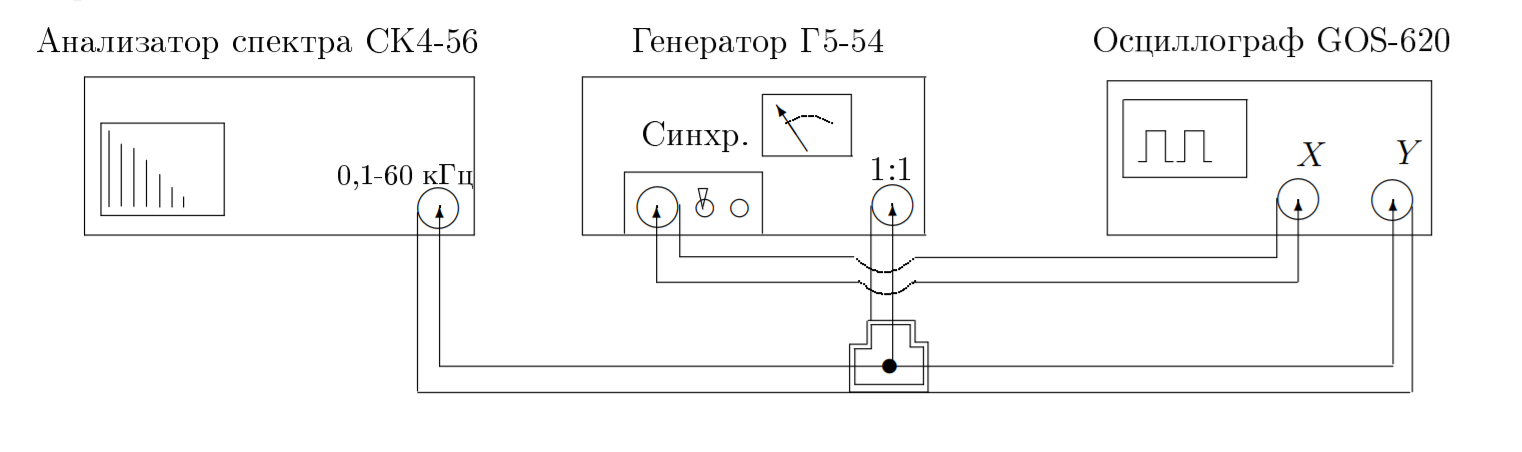
\includegraphics[width=\linewidth]{sp7.png}
			\caption{Cхема для исследования спектра периодической последовательности прямоугольных импульсов}
			\label{A}
		\end{figure}
			
		\item \textbf{Экспериментальная установка Б} для исследования спектра периодической последовательности цугов гармонических колебаний (рис. 8) Генератор Г6-34 вырабатывает синусоидальные колебания высокой частоты. На вход АМ (амплитудная модуляция) генератора Г6-34 подаются прямоугольные импульсы с генератора Г5-54 и синусоида модулируется - "нарезается" на отдельные куски - цуги. Эти цуги с выхода генератора Г6-34 поступают на вход спектроанализатора и одновременно на вход Y осциллографа. Сигнал синхронизации подается на осциллограф с генератора импульсов.
		
		\newpage
		
		\begin{figure}[h]
			\centering
			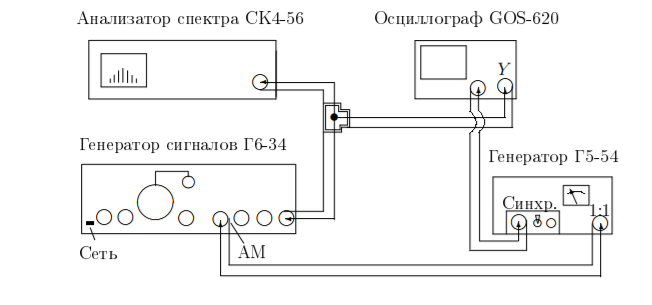
\includegraphics[width=0.8\linewidth]{sp8.png}
			\caption{Cхема для исследования спектра периодической последовательности цугов высокочастотных колебаний}
			\label{B}
		\end{figure}
		
		\item \textbf{Экспериментальная установка В} для исследования амплитудно - модулированного сигнала (рис. 9). В генератор сигналов встроен модуляционный генератор, который расположен в левой части Г6-34. Синусоидальный сигнал с частотой модуляции $f_{мод}=1$ кГц подается с модуляционного генератора на вход АМ (амплитудная модуляция) генератора, вырабатывающего синусоидальный сигнал высокой частоты (частота несущей $\nu_{0}=25$ кГц). Амплитудно-модулированный сигнал с основного выхода генератора поступает на осциллограф и на анализатор спектра. 
		
		\begin{figure}[h]
			\centering
			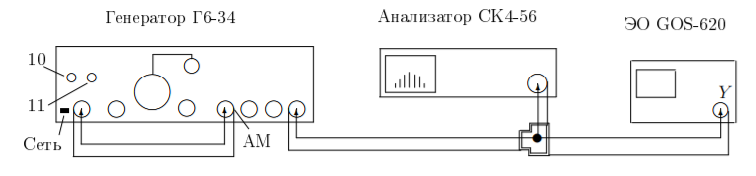
\includegraphics[width=0.8\linewidth]{sp9.png}
			\caption{Cхема для исследования спектра высокочастотного гармон. сигнала, промодулированного по амплитуде низкочастотным гармон. сигналом}
			\label{C}
		\end{figure}
	\end{enumerate}

  	\section{Ход работы}
  	
  	\subsection{Исследование спектра периодической последовательности прямоугольных импульсов}
  	
  	Соберем схему согласно рис. 7 и включим в сеть только генератор Г5-54.
 	Установив на анализаторе режим работы с однократной развјрткой, по-
  	лучим на его экране спектр импульсов с параметрами $ f_{повт}  = 103 $ Гц;
  $ \tau= 25 $ мкс; частотный масштаб $ m_x = 5 $ кГц/дел. Полученная картина представлена на рис. \ref{A_or}. 
  
  \begin{figure}[h]
  	\centering
  	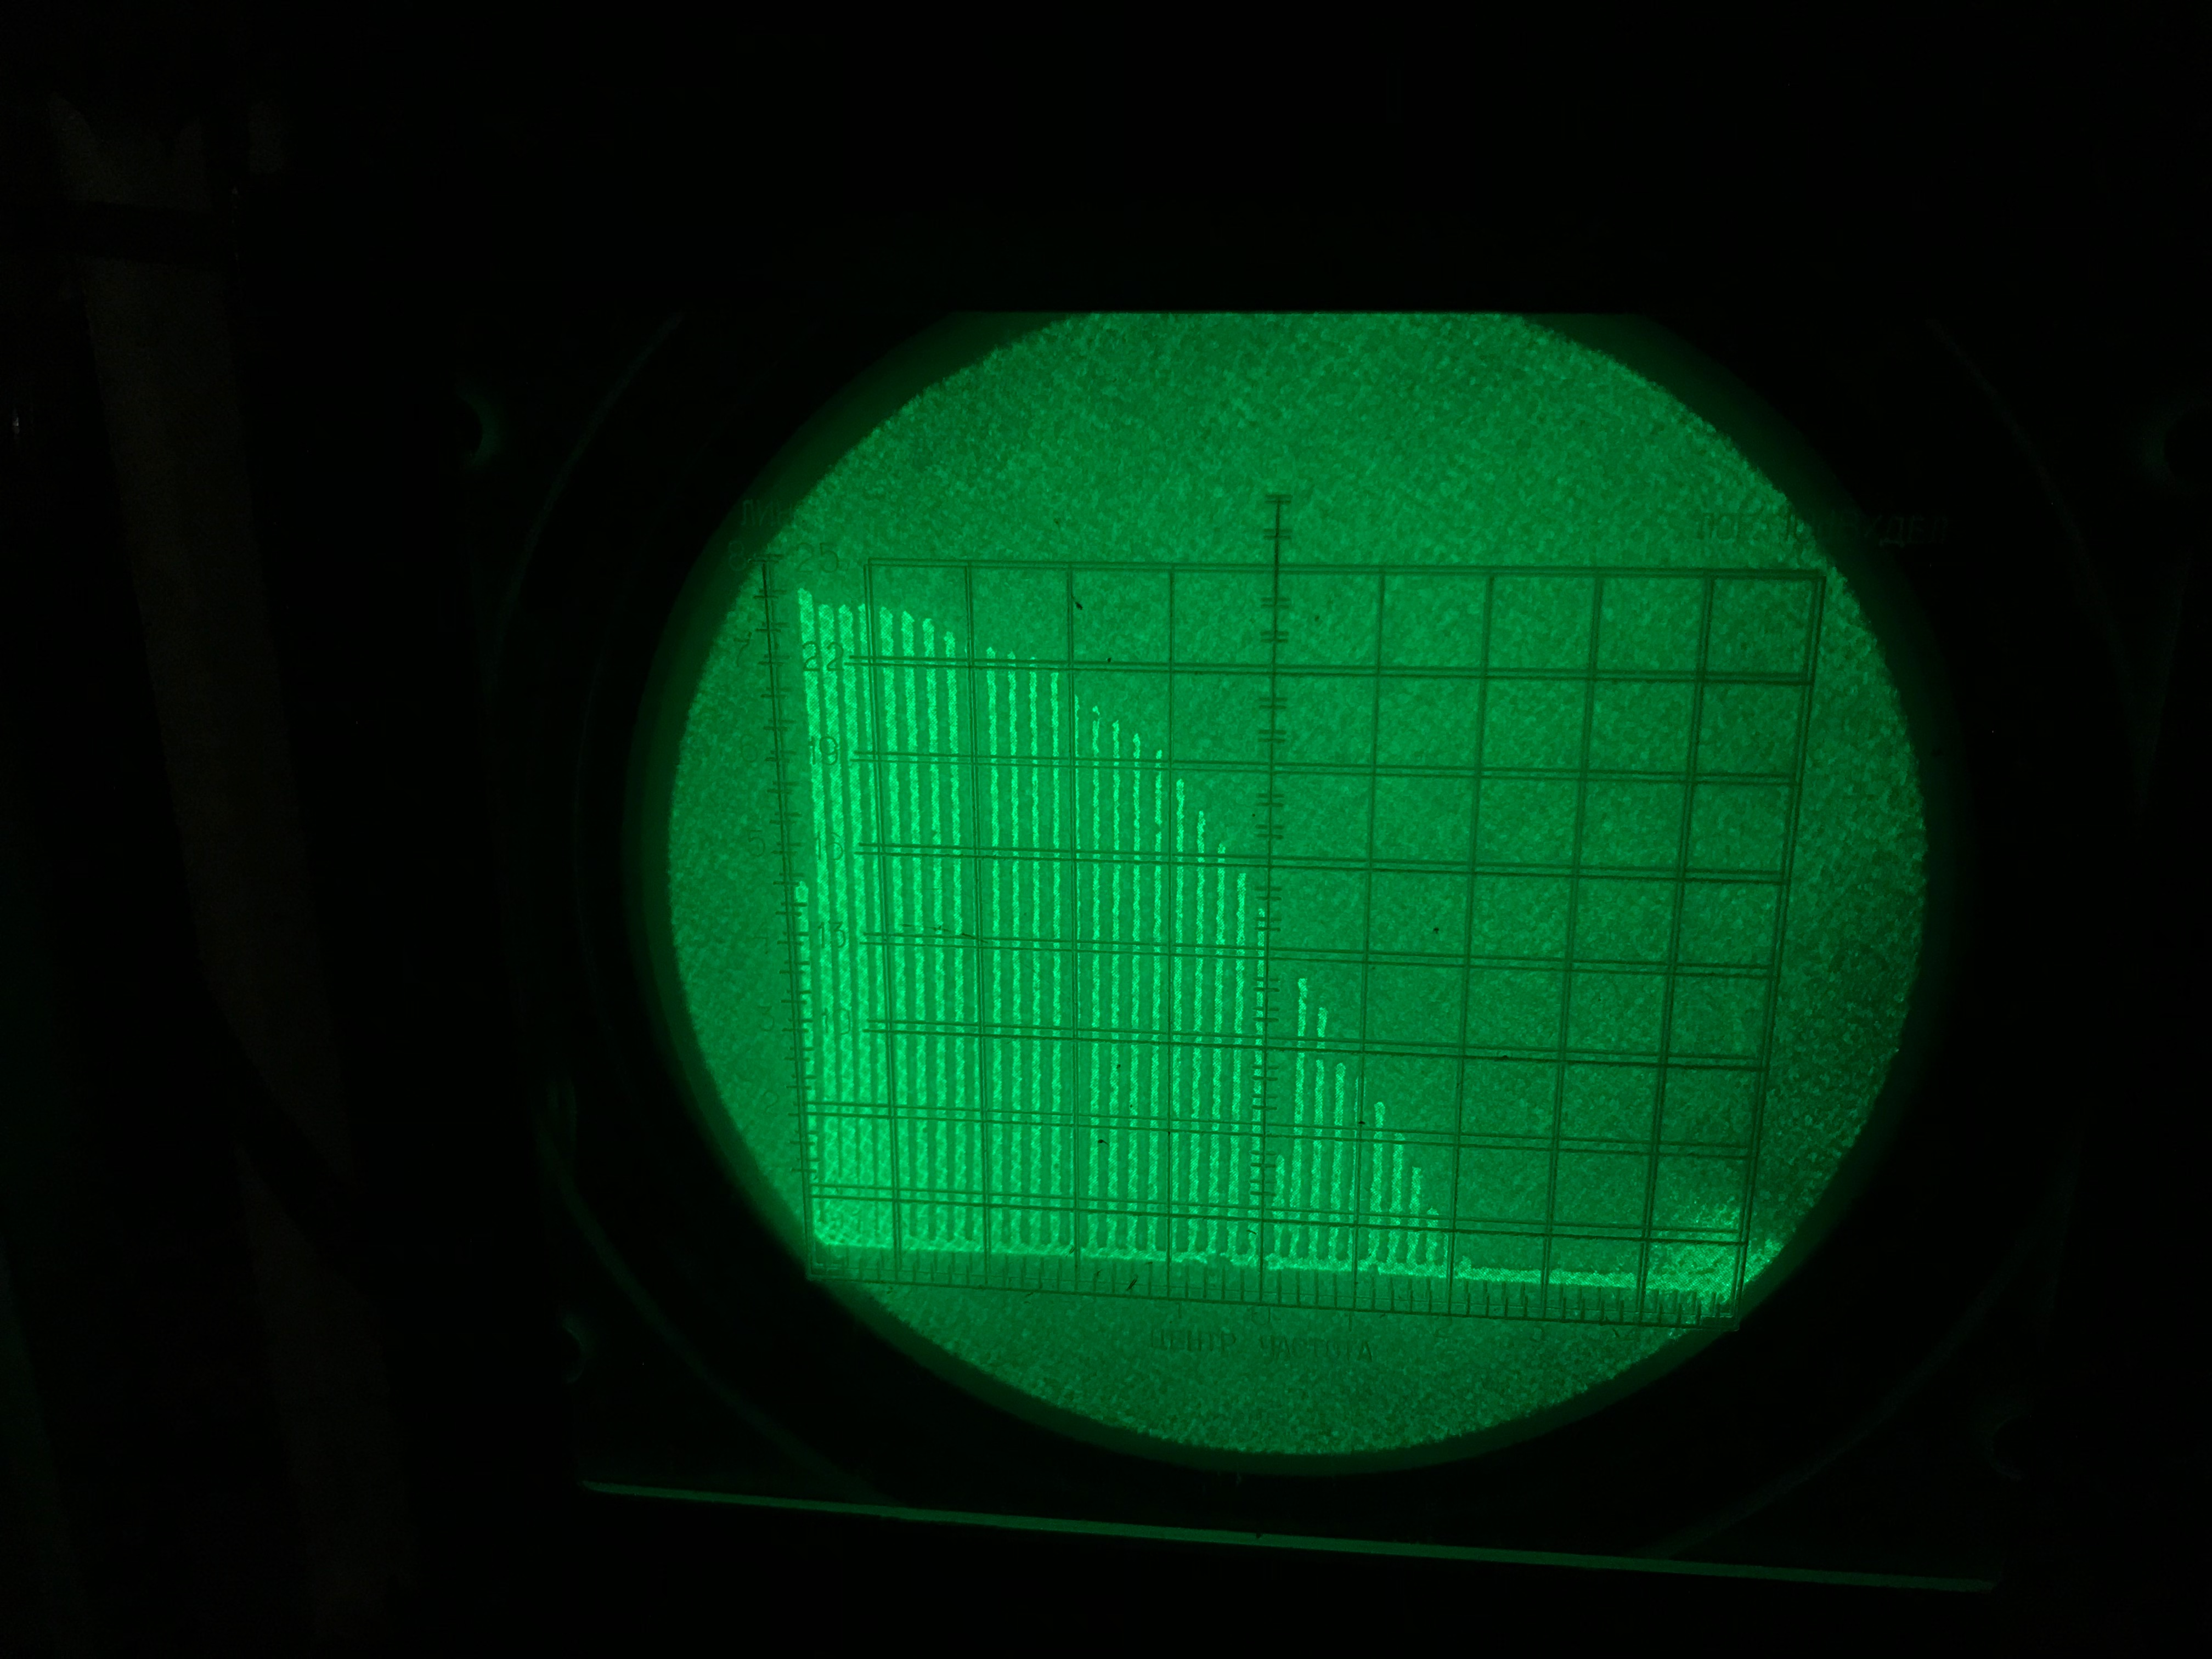
\includegraphics[width=0.65\linewidth]{A_or.jpg}
  	\caption{Спектр прямоугольных импульсов}
  	\label{A_or}
  \end{figure}
  
  При увеличении длительности импульсов $ \tau $ вдвое на экране получаем следующую картину (рис. \ref{A_tau}), а при увеличении вдвое $ f_{повт} $ --- рис. \ref{A_f}. Таким образом, в первом случае уменьшилась ширина спектра, а во втором --- увеличилось расстояние между компонентами спектра.
  
  Теперь проведем измерения зависимости ширины спектра от длительности импульсов, оставляя неизменным $ f_{повт} = 1 $ кГц. Результаты занесем в таблицу \ref{A_table}. Построим график зависимости $ \Delta \nu \left (\dfrac{1} {\tau} \right ) $. 
  \begin{figure}[h!]
  	\begin{minipage}[h]{0.5\linewidth}
  		\center{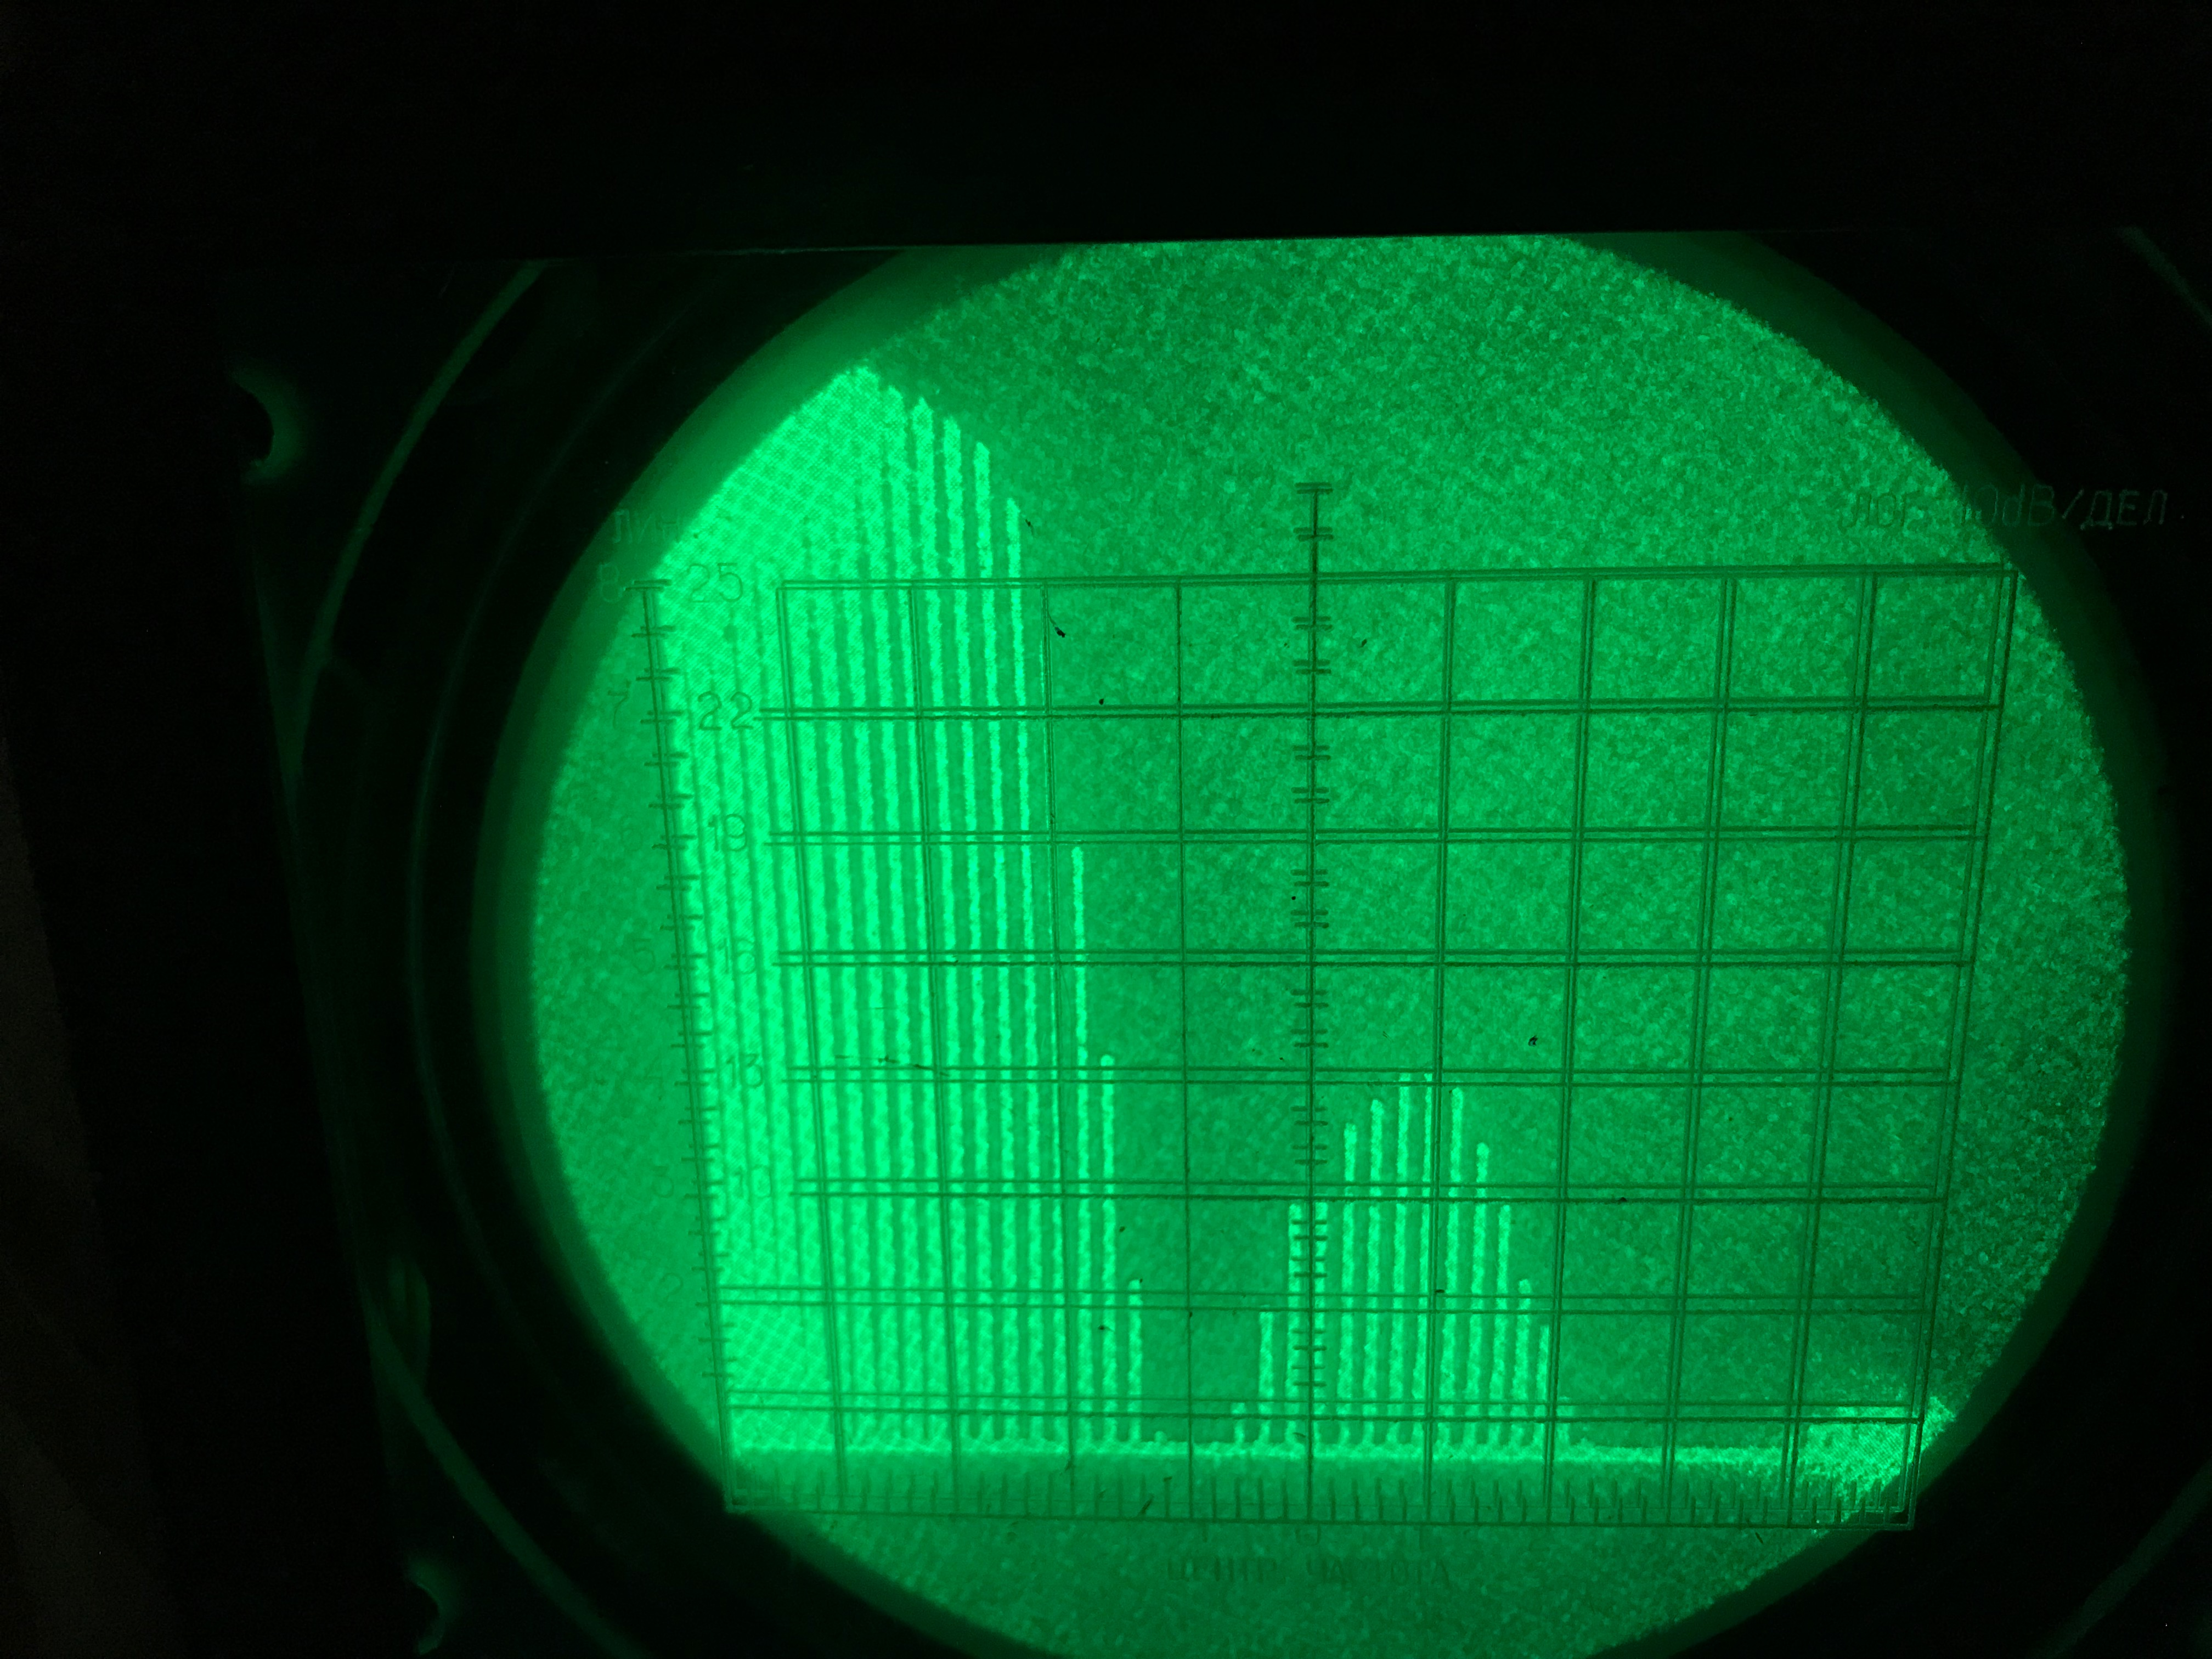
\includegraphics[width=0.9\linewidth]{A_tau.jpg}}
  		\caption{Спектр прямоугольных импульсов при $\tau$=50 мкс}
  		\label{A_tau}
  	\end{minipage}
  	\begin{minipage}[h]{0.5\linewidth}
  		\center{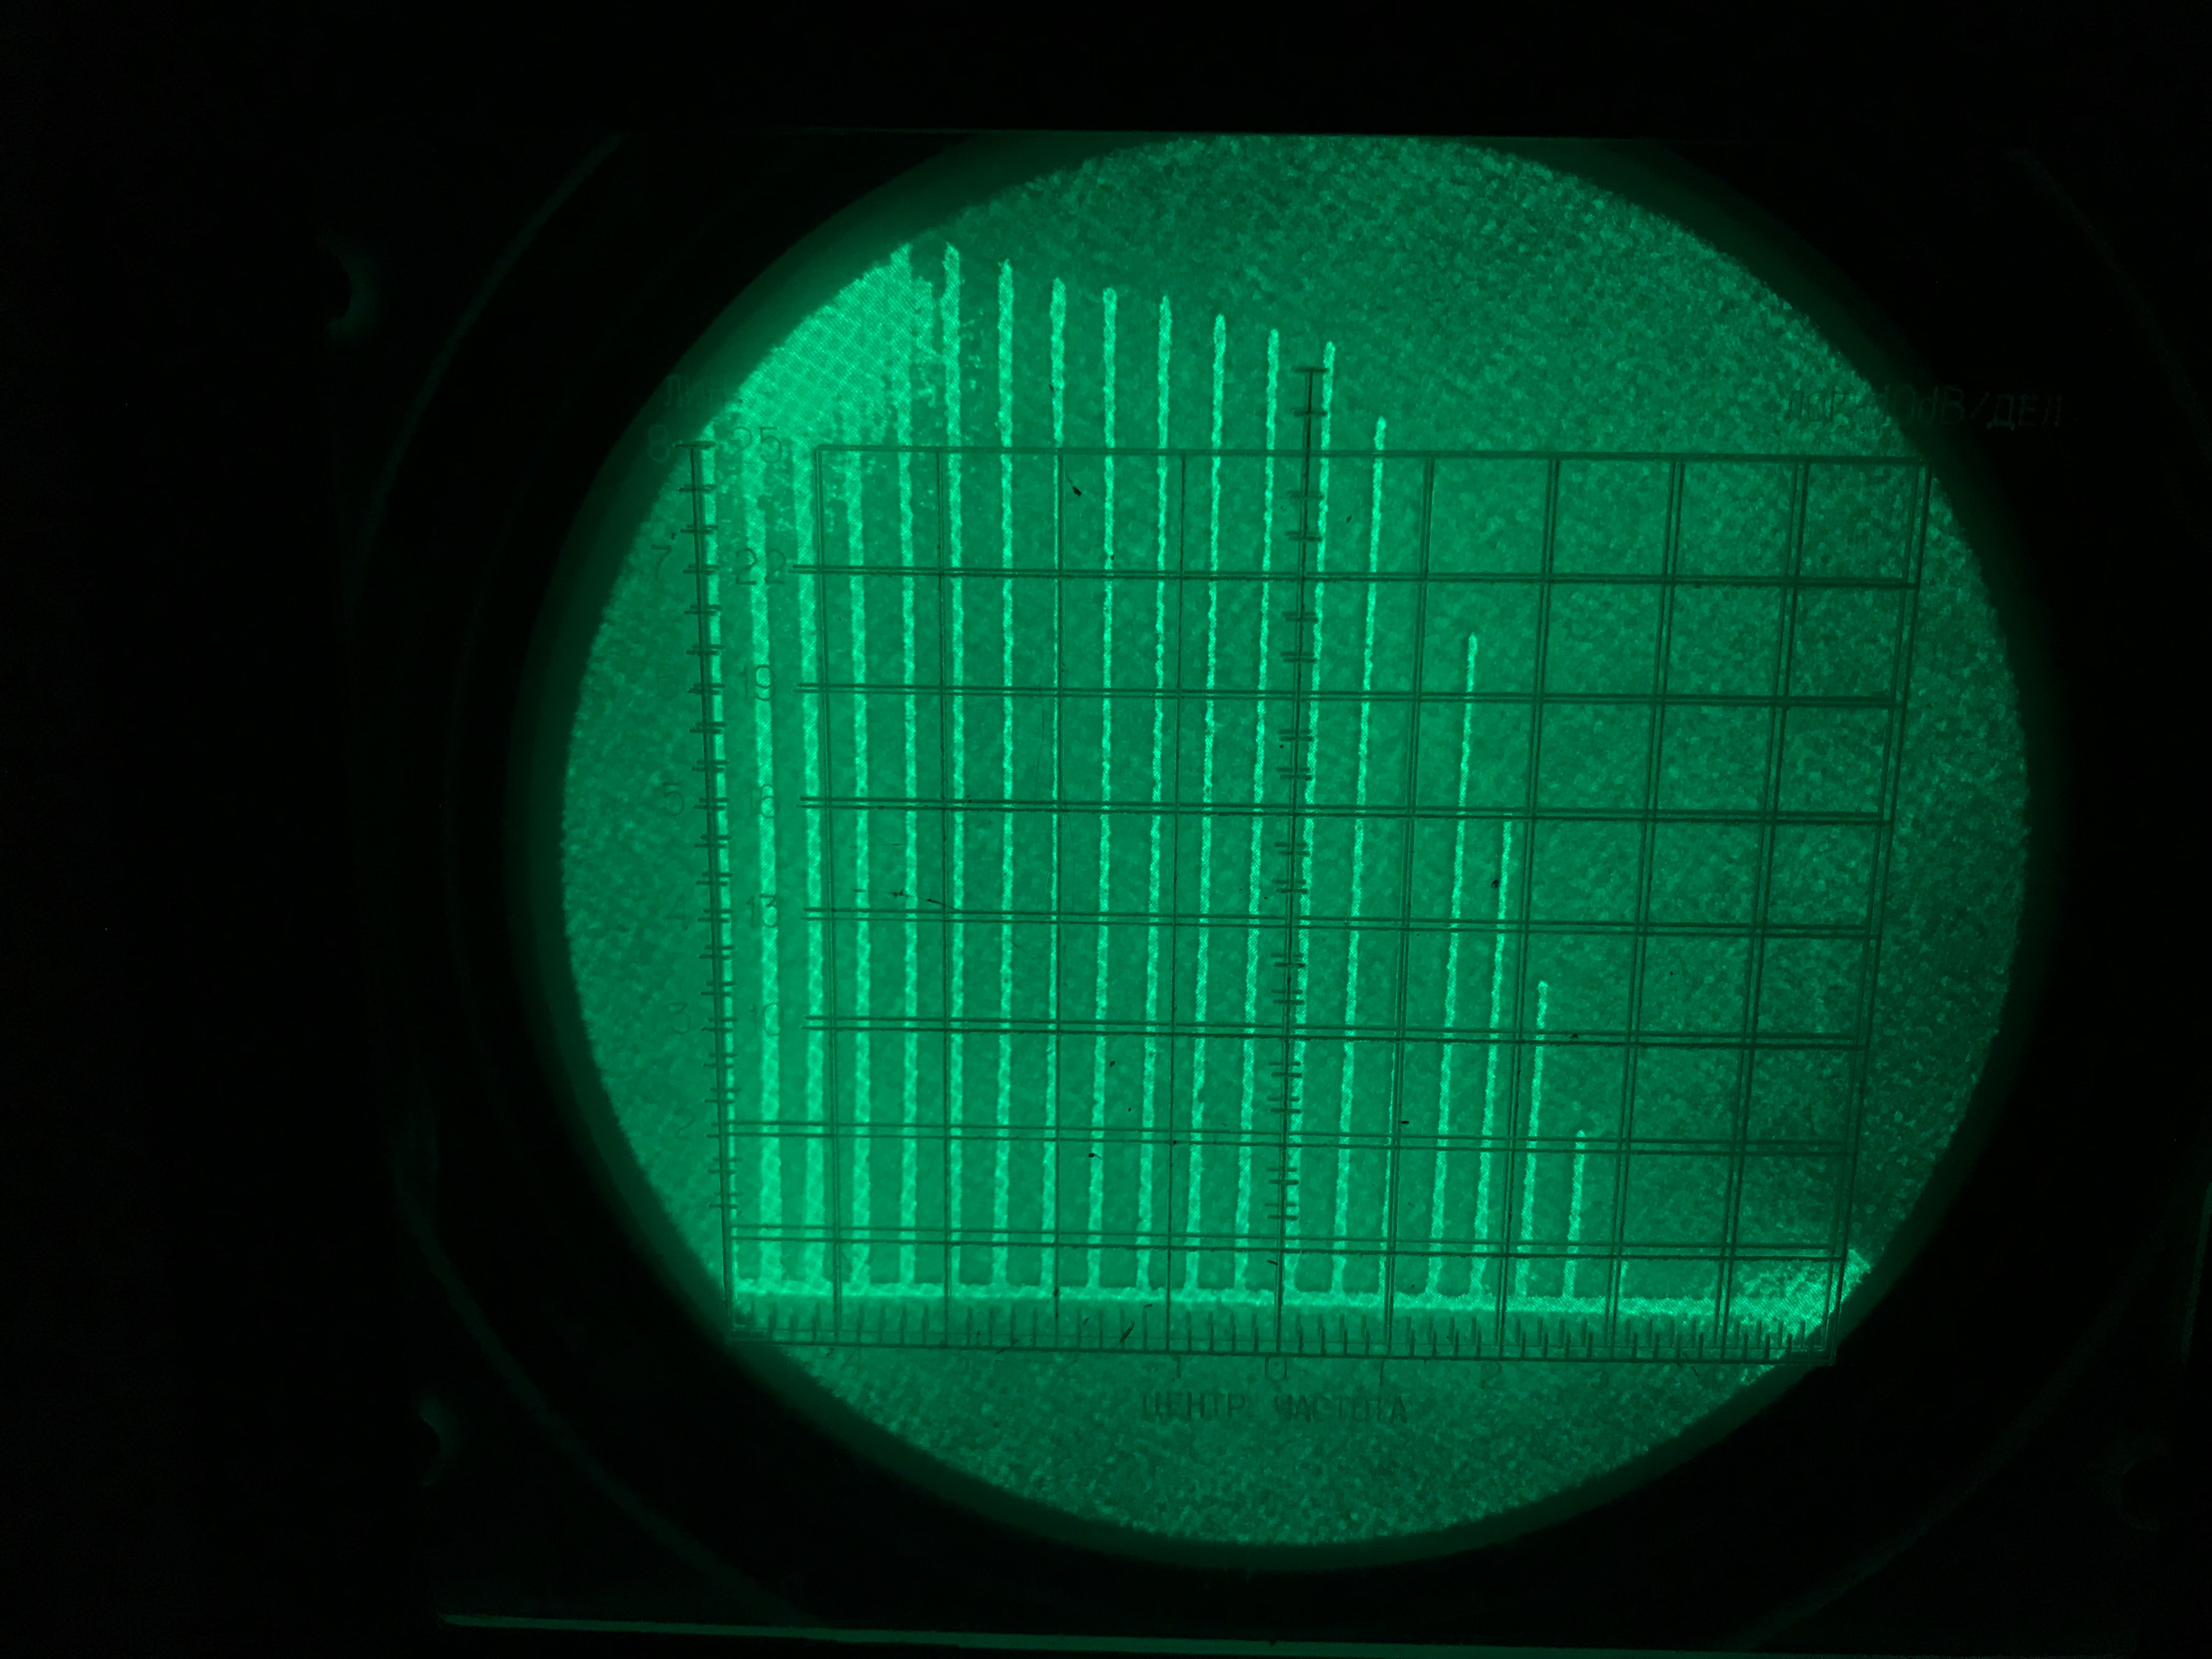
\includegraphics[width=0.9\linewidth]{A_ff.jpg}}
  		\caption{Спектр прямоугольных импульсов при $f_{повт}=2$ кГц}
  		\label{A_f}
  	\end{minipage}
  \end{figure}
  	
  	\begin{table}[]
  		\caption{Зависимость ширины спектра от длительности импульсов}
  		\begin{center}
  			\begin{tabular}{|c|c|c|c|}
  			\hline
  			$ N $ & $ \tau $, мкс & $ \Delta\nu, $ кГц  & $ \dfrac{1}{\tau}, \; 10^{-3} \; мкс^{-1}$ \\
  			\hline
  			1. & 32. & 31.0 & 31.3 \\
  			2 & 50 & 19.0 & 20.0 \\
  			3 & 70 & 12.5 & 14.3 \\
  			4 & 90 & 10.0 & 11.1 \\
  			5 & 120 & 7.0 & 8.3 \\
  			6 & 150 & 6.0 & 6.7 \\
  			7 & 175 & 4.5 & 5.7 \\
  			8 & 200 & 3.5 & 5.0 \\
  				\hline
  			\end{tabular}
  		\end{center}
  	\label{A_table}
  	\end{table}
  	
  	\begin{figure}[h!]
  		\label{A_graf}
  		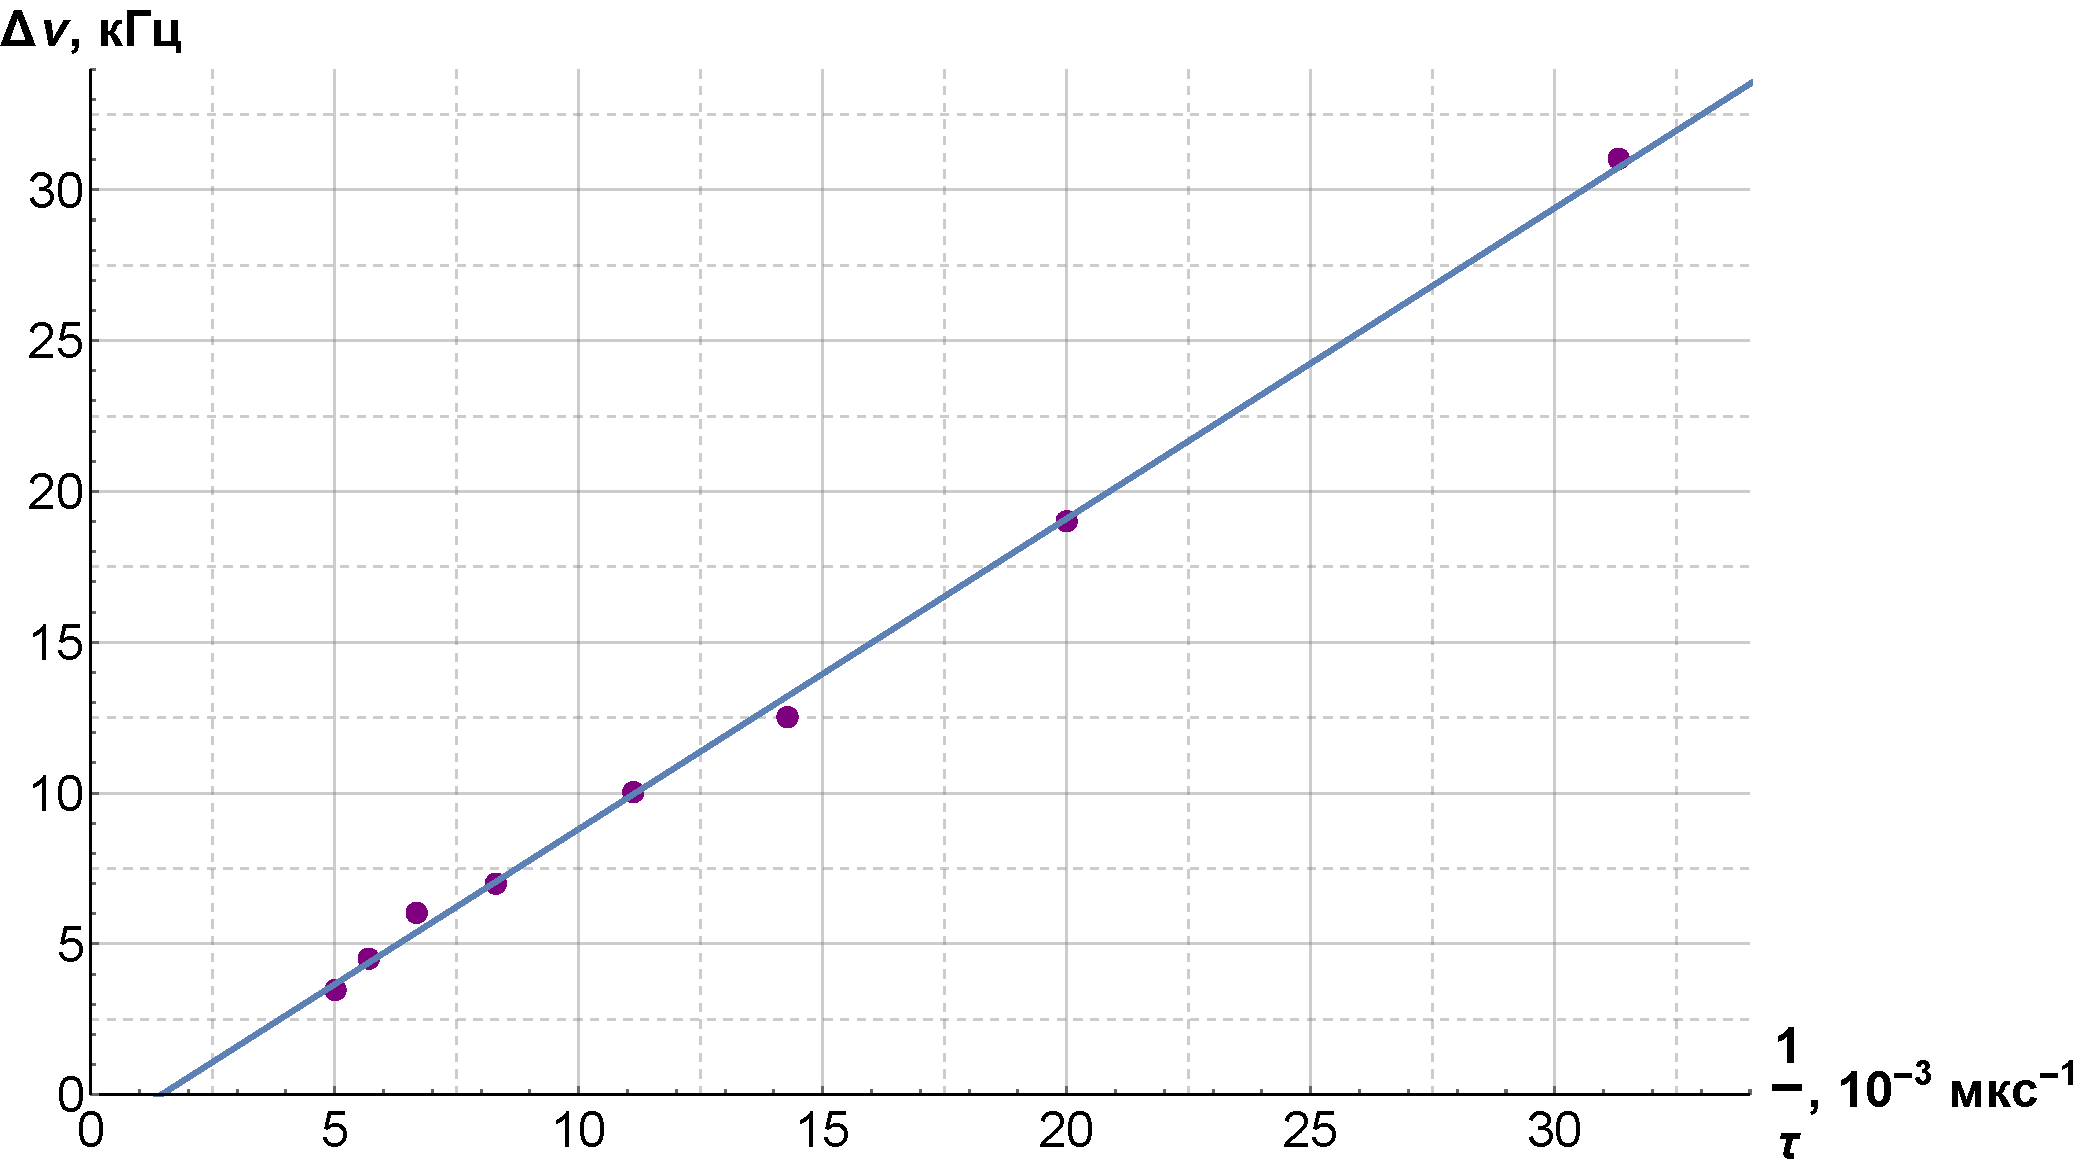
\includegraphics[scale=0.47]{A.pdf}
  		\caption{График зависимости $ \Delta \nu \left (\dfrac{1}{\tau} \right ) $. }
  	\end{figure}
  	
  	\begin{table}[h!]
  		\centering
  		\caption{Расчет апроксимированной прямой $ y = ax +b $}
  		\begin{tabular}{c|cc}
  			\text{} & \text{Estimate} & \text{Standard Error} \\
  			\hline
  			a & 1.029 & 0.017  \\
  			b & -1.497 & 0.268  \\
  		\end{tabular}
  	\end{table}
  
  	
  	Из него (рис \ref{A_graf}) получем коэффициент наклона аппроксимированной прямой $ y = ax + b $:  
  	
  	\begin{equation}\label{}
  	a = 1,029 \pm 0,017 
  	\end{equation}
  	
  	Это соответствует соотношению неопределённости \eqref{neopr}. 
  	
  	\subsection{Исследование спектра периодической последовательности цугов гармонических колебаний}
  	
  	Соберём схему, изображённую на рис. \ref{B}. Установив частоту несущей $ \nu_0 = 25  $ кГц, посмотрим, как изменяется вид спектра при увеличении длительности импульса вдвое (т.е. при $ \tau = 50, \; 100 $ мкс, $ f_{повт} = 1 $ кГц). Получаем, что ширина спектра уменьшится, а модули спектра (амплитуда) увеличится. 
  	
  	 \begin{figure}[h]
  		\centering
  		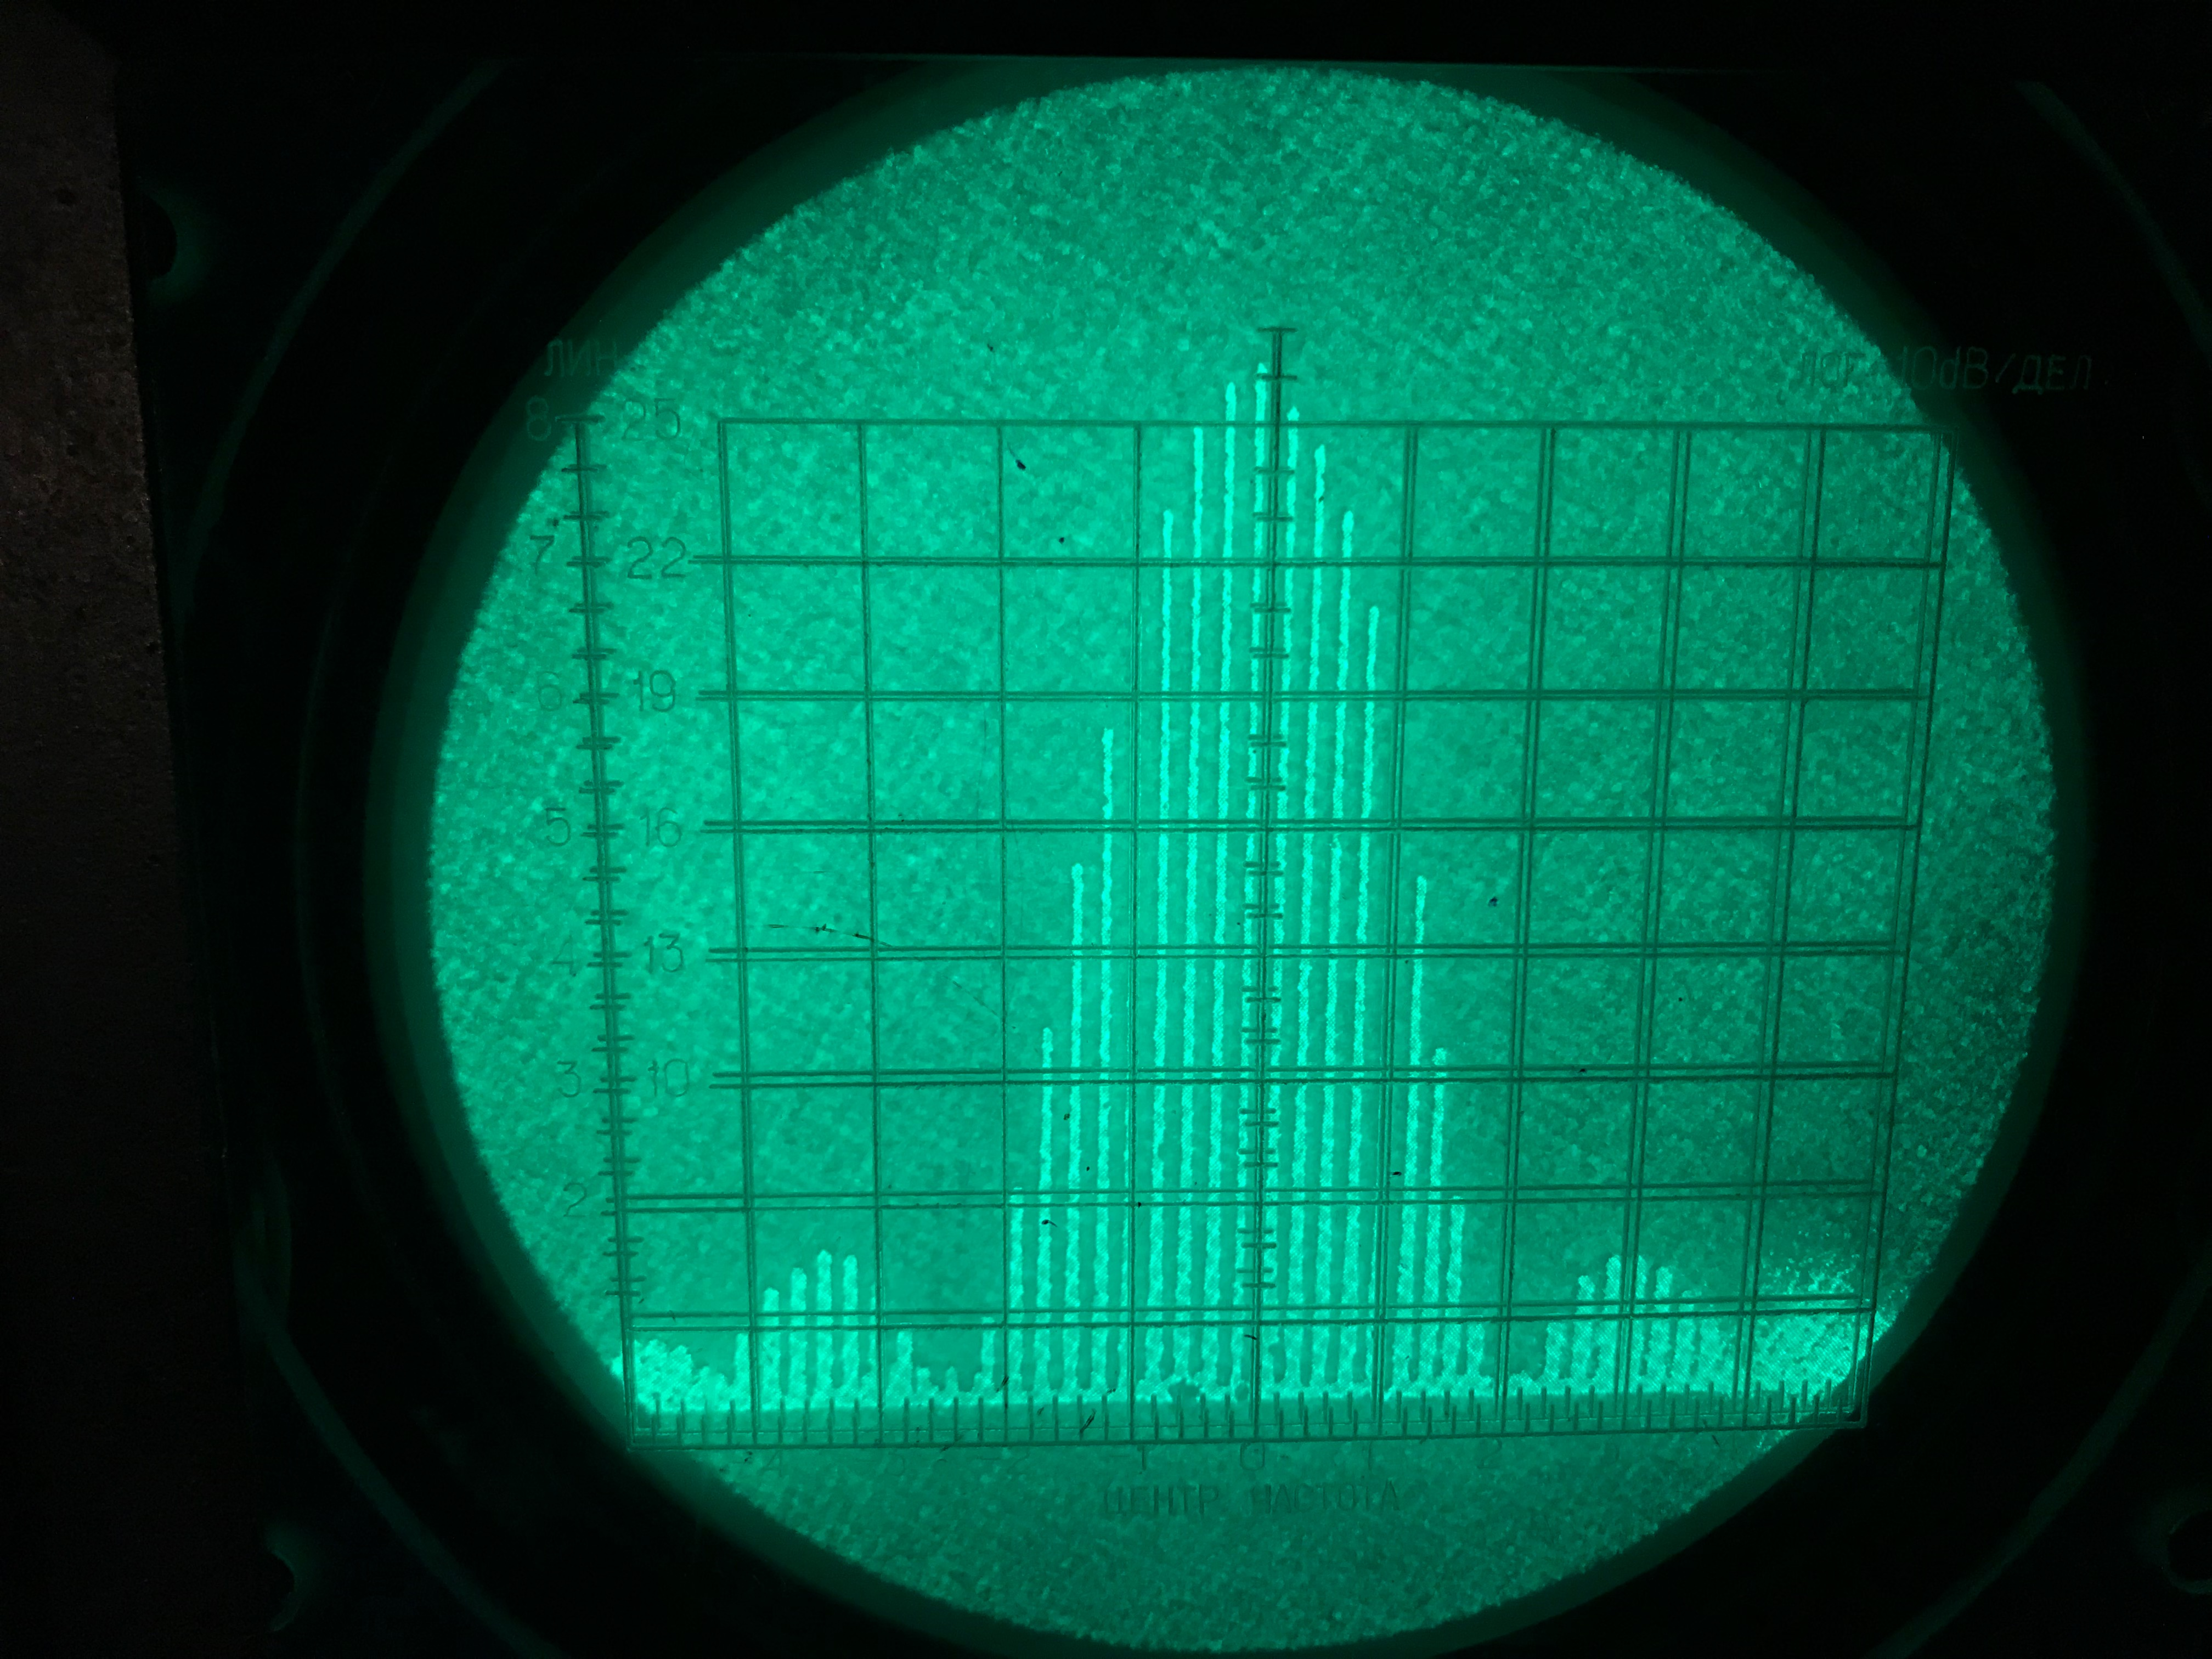
\includegraphics[width=0.65\linewidth]{B_25.jpg}
  		\caption{Спектр при частоте несущей $ \nu_0 = 25 $ кГц}
  		\label{B_25}
  	\end{figure}
  	
  	При фиксированных значениях $  f_{повт} = 1 $ кГц, $ \tau= 100 \; мкс $ и частотном масштабе $ m_x = 5  $кГц/дел посмотрим, как меняется картина спектра при изменении несущей частоты $ \nu_0 $ (на генераторе Г6-34 $ \nu_0 = 10, 25, 40 $ кГц.). Результаты отразим на рисунках \ref{B_25} -- \ref{B_40}. 
  	
  	\begin{figure}[h!]
  		\begin{minipage}[h]{0.5\linewidth}
  			\center{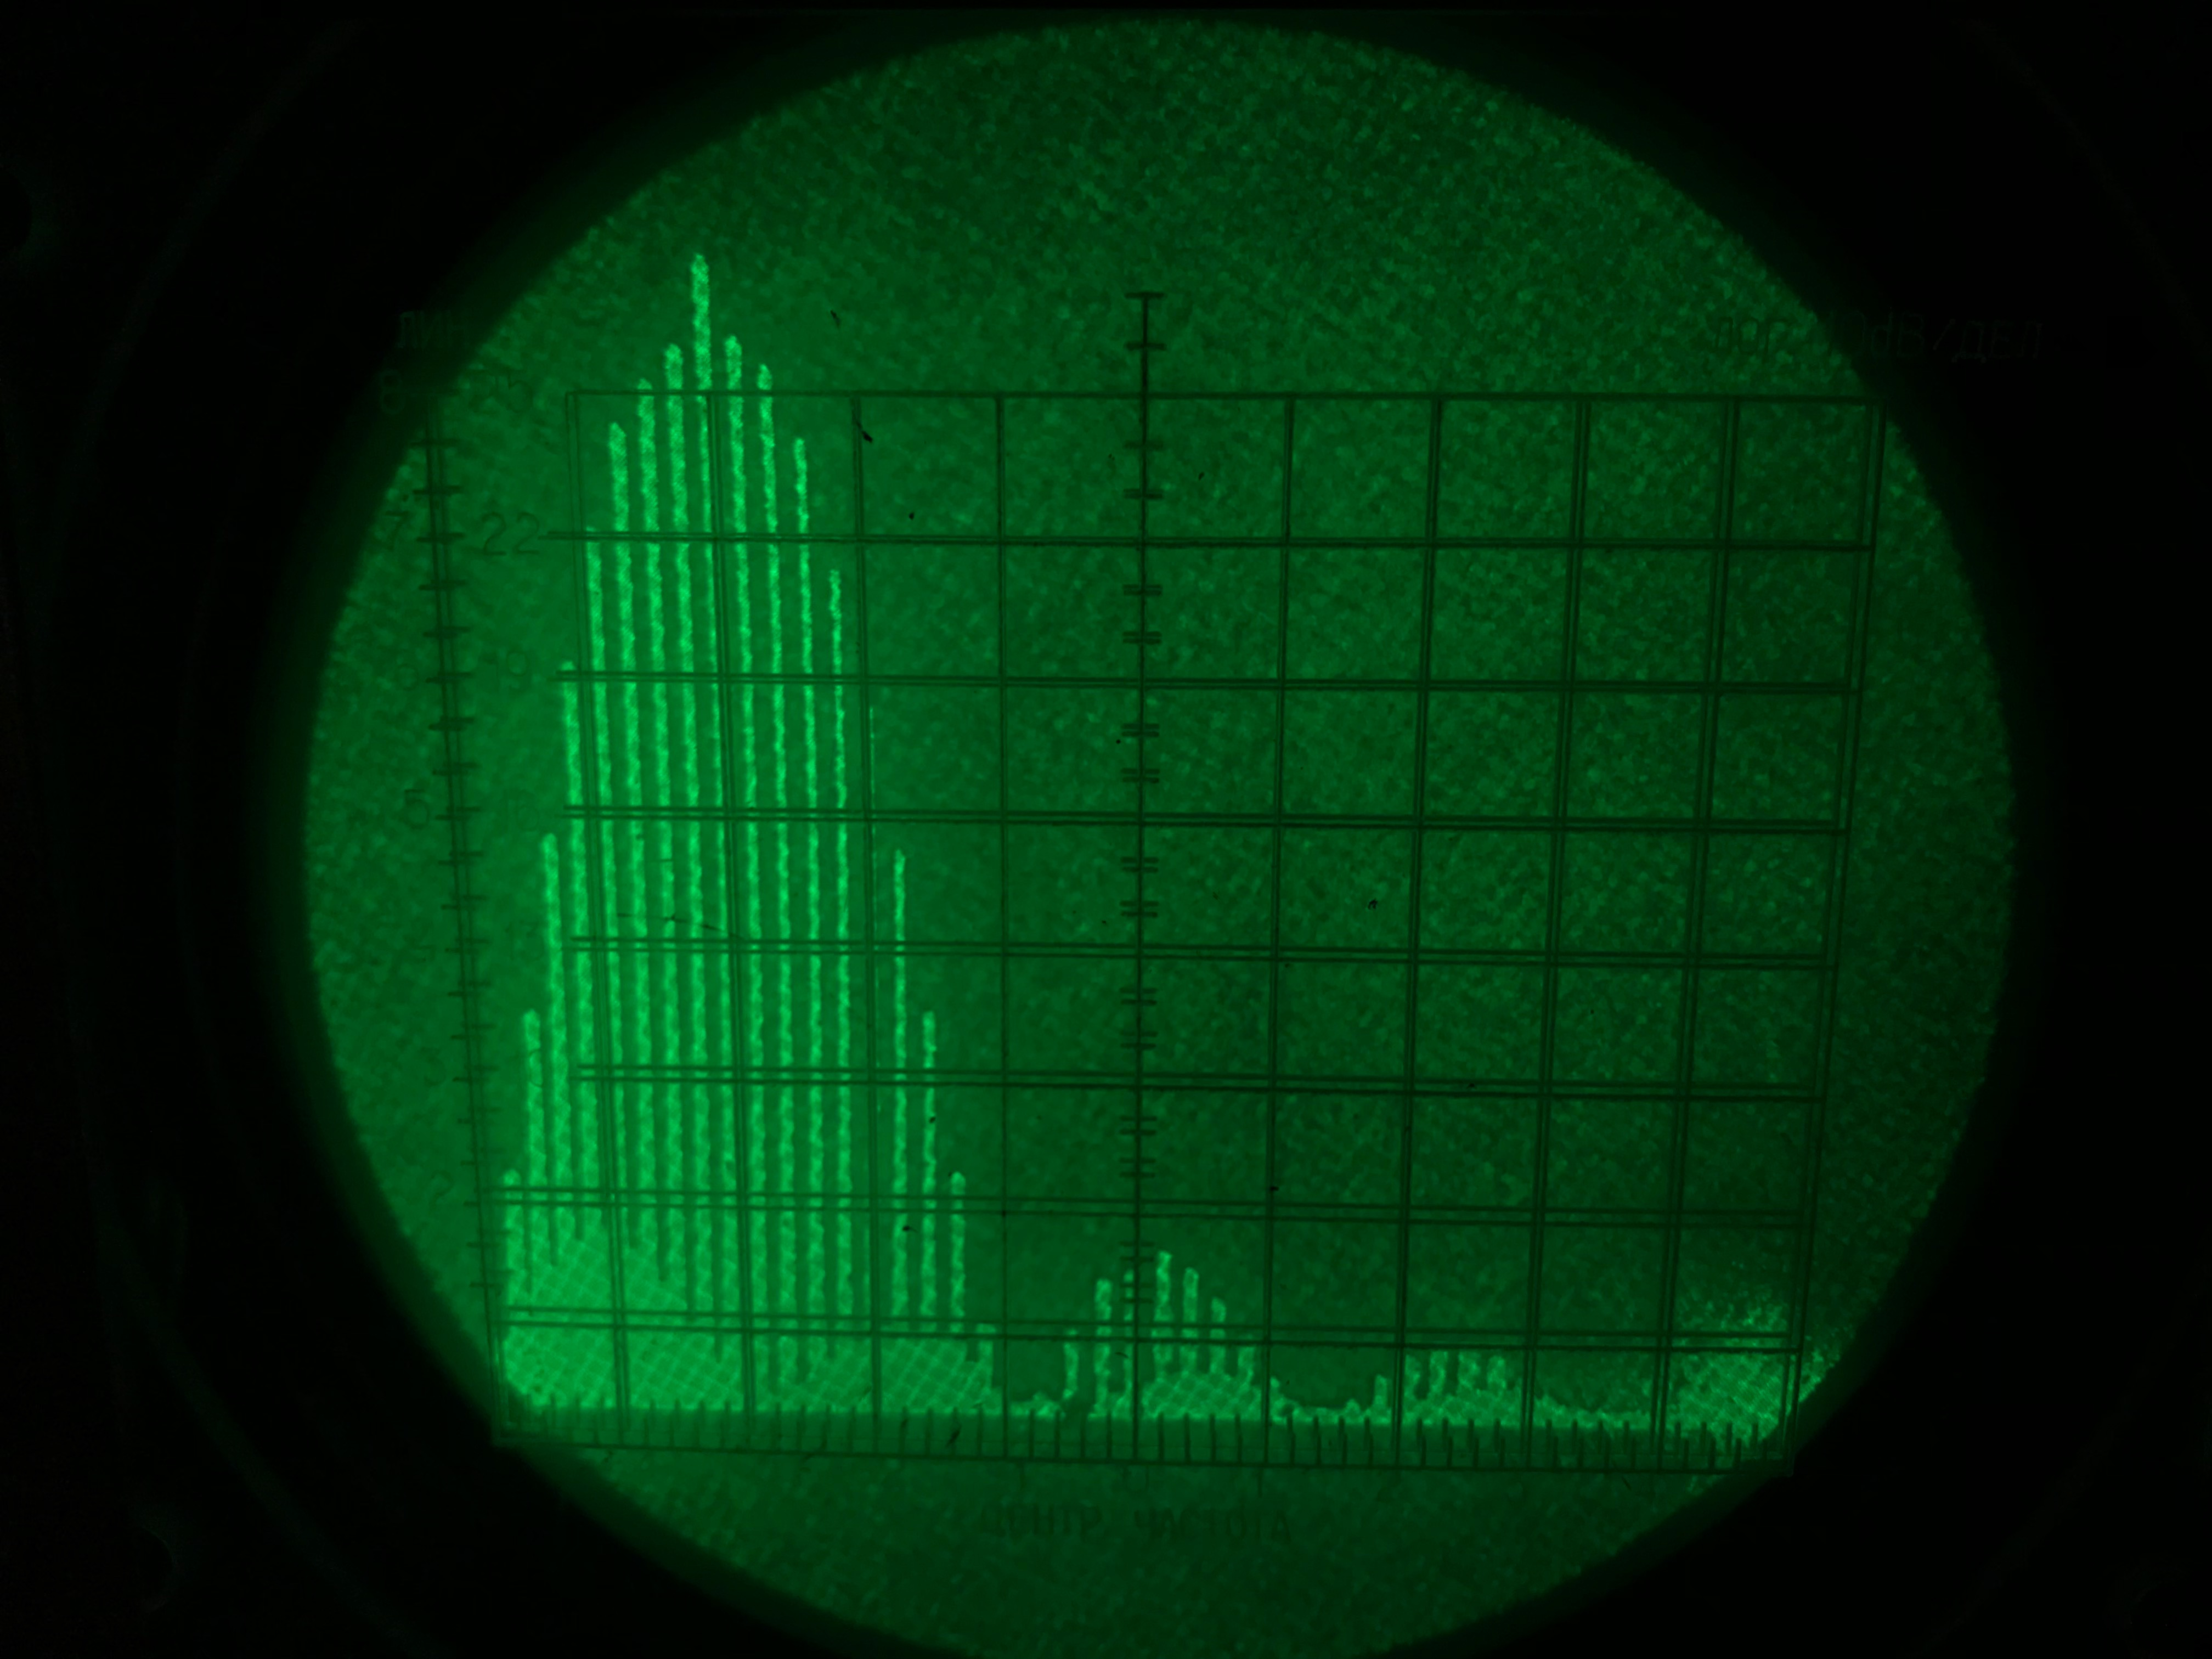
\includegraphics[width=0.9\linewidth]{B_10.jpg}}
  			\caption{Спектр при частоте несущей $ \nu_0 = 10 $ кГц}
  			\label{B_10}
  		\end{minipage}
  		\begin{minipage}[h]{0.5\linewidth}
  			\center{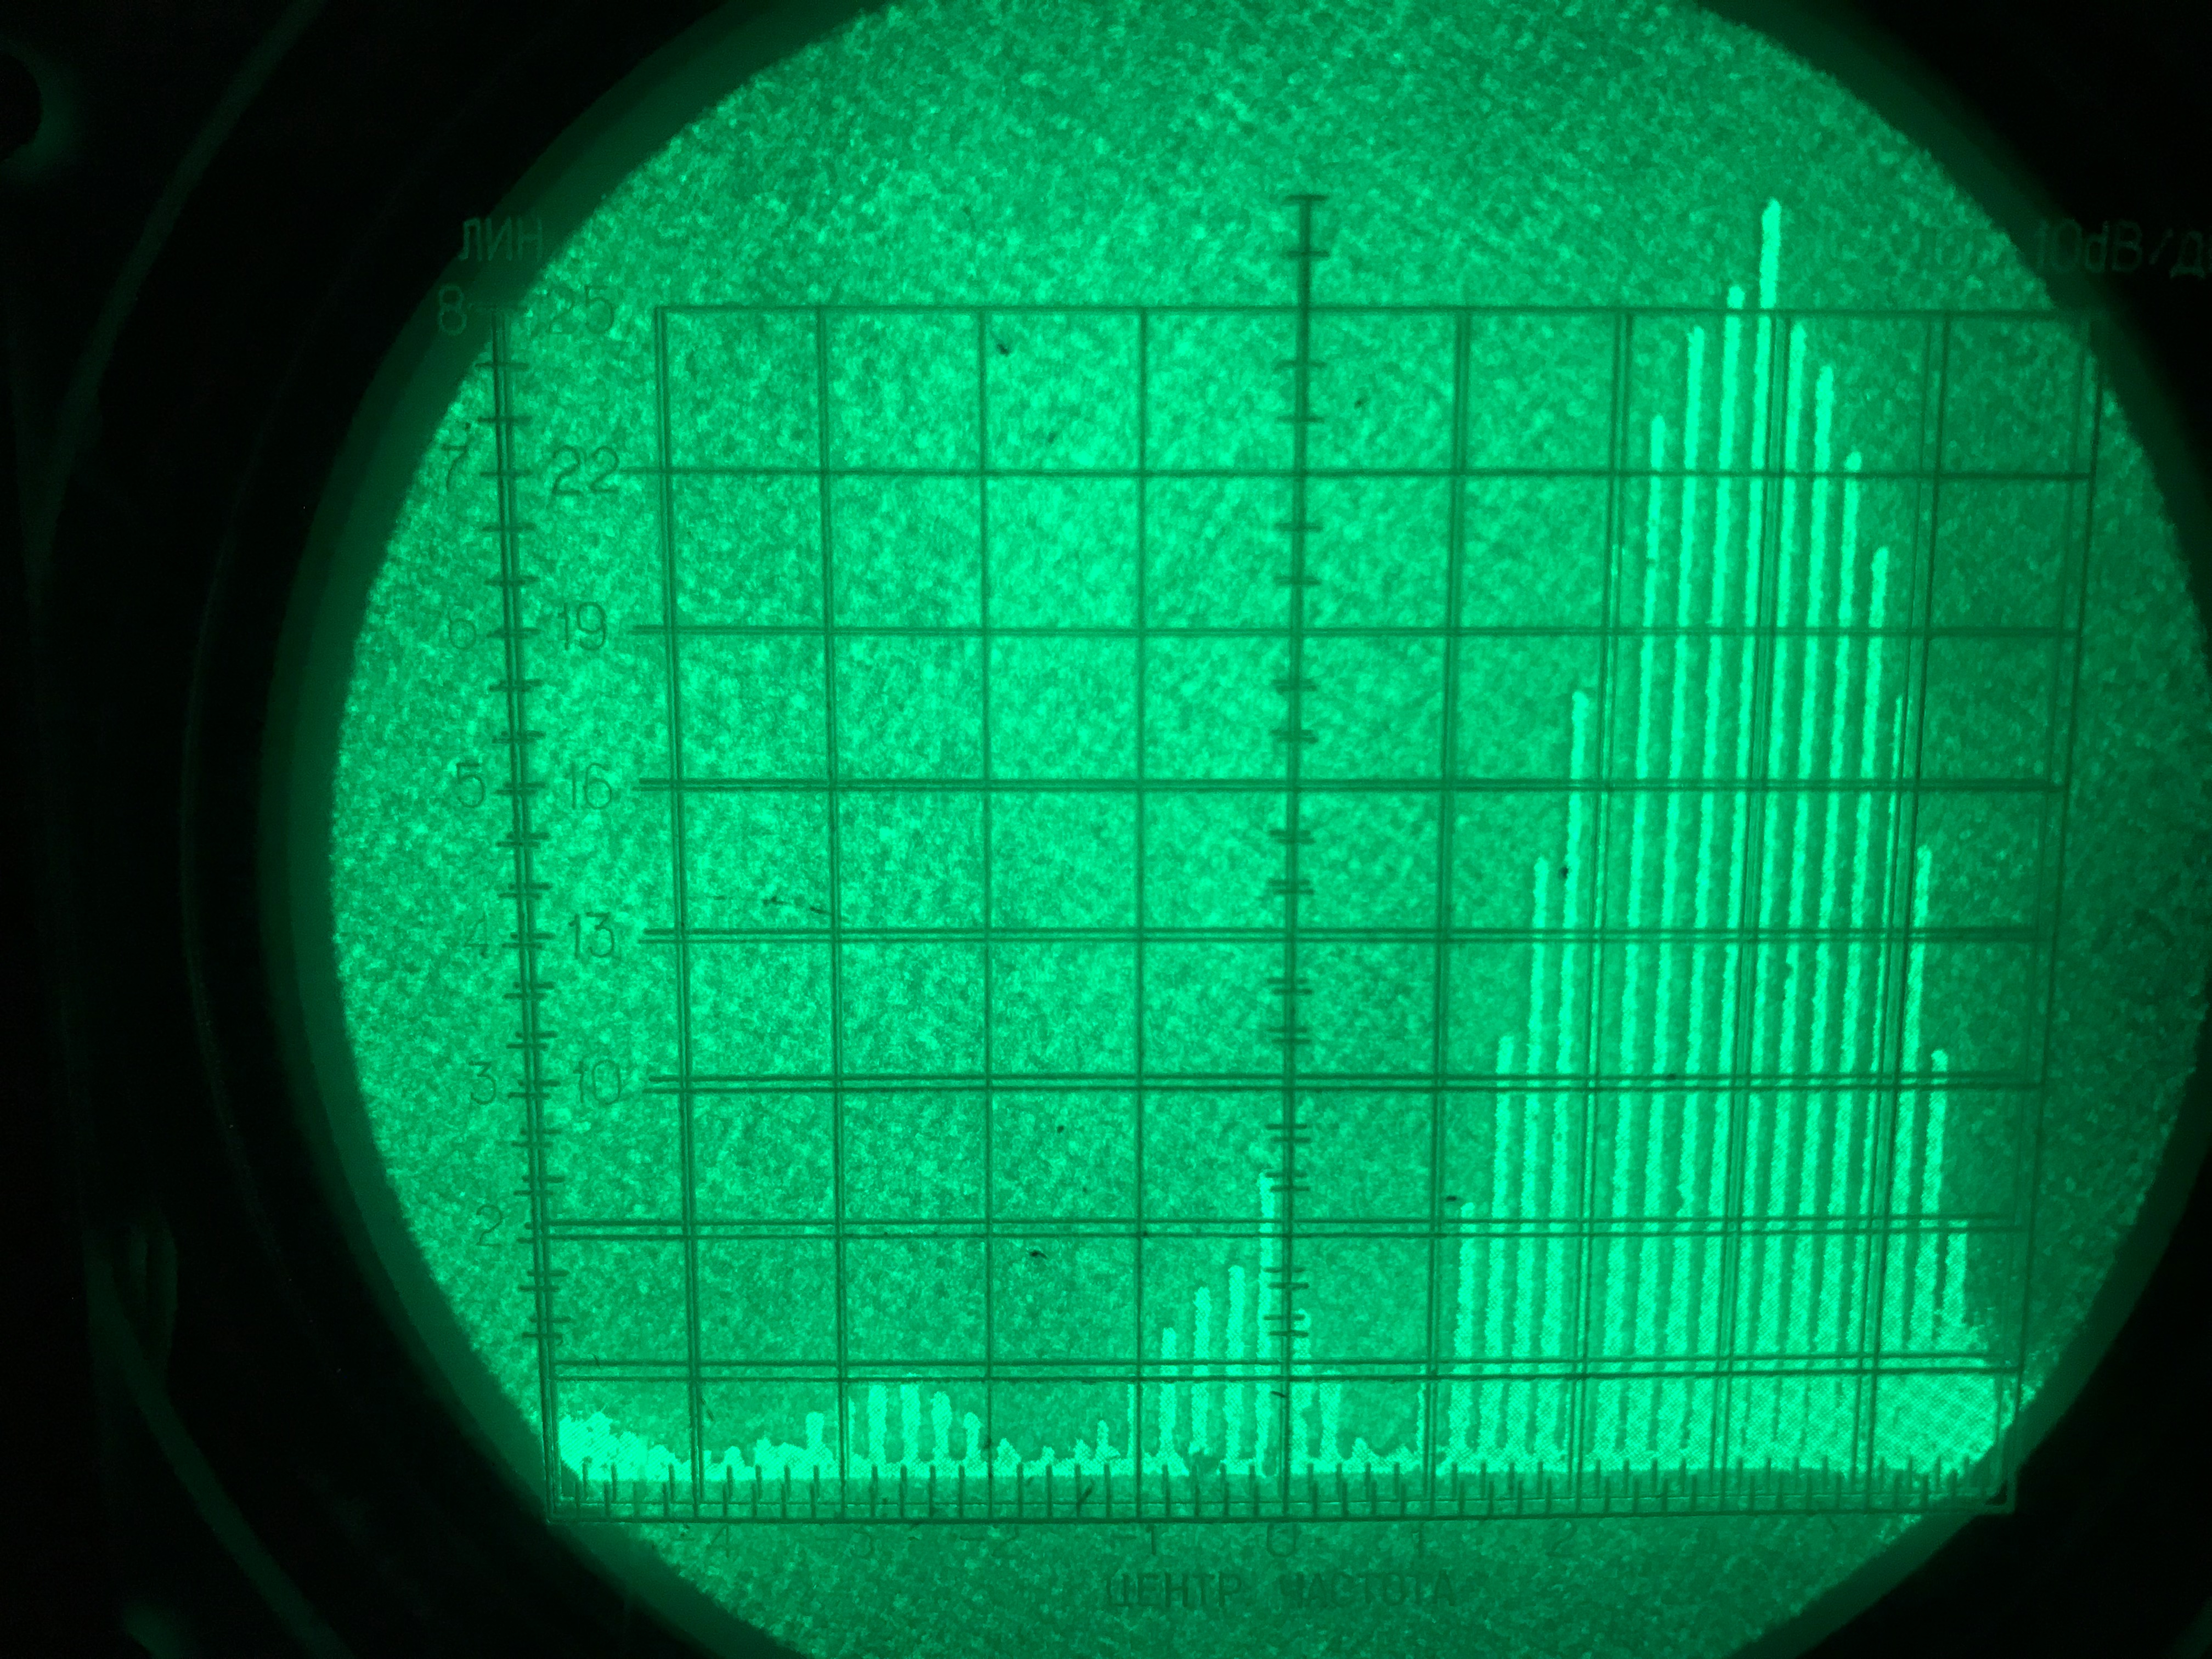
\includegraphics[width=0.9\linewidth]{B_40.jpg}}
  			\caption{Спектр при частоте несущей $ \nu_0 = 40 $ кГц}
  			\label{B_40}
  		\end{minipage}
  	\end{figure}
  	
  	При фиксированной длительности импульсов  $ \tau = 50 $ мкс исследуем зависимость расстояния между соседними спектральными компонентами
  	от периода $ T $ (частоты повторения импульсов $ f_{повт} $). Проведем измерения для 5 -- 6 значений частоты $ f_{повт} $ в диапазоне 1 -- 8 кГц, подбирая горизонтальный масштаб mx, удобный для измерений. Результаты занесем в таблицу \ref{B_table} и построим график зависимости расстояния между компонентами спектра $ \delta \nu $ от частоты повторения импульсов $ f_{повт} $ (рис \ref{B_graf}). 
  
  	\begin{table}[]
  		\caption{Зависимость расстояния между компонентами спектра $ \delta \nu $ от частоты повторения импульсов $ f_{повт} $}
  		\begin{center}
  			\begin{tabular}{|c|c|c|}
  				\hline
  				$ N $  & $ f_{повт}, $ кГц  & $ \delta \nu $, кГц \\
  				\hline
  				1 & 1.0 & 1.2 \\
  				2 & 2.0 & 2.3 \\
  				3 & 3.5 & 3.7 \\
  				4 & 5.0 & 5.6 \\
  				5 & 6.5 & 7.2 \\
  				6 & 8.0 & 9.0 \\
  				\hline
  			\end{tabular}
  		\end{center}
  		\label{B_table}
  	\end{table}
  	
  	\begin{figure}[h!]
  		\label{B_graf}
  		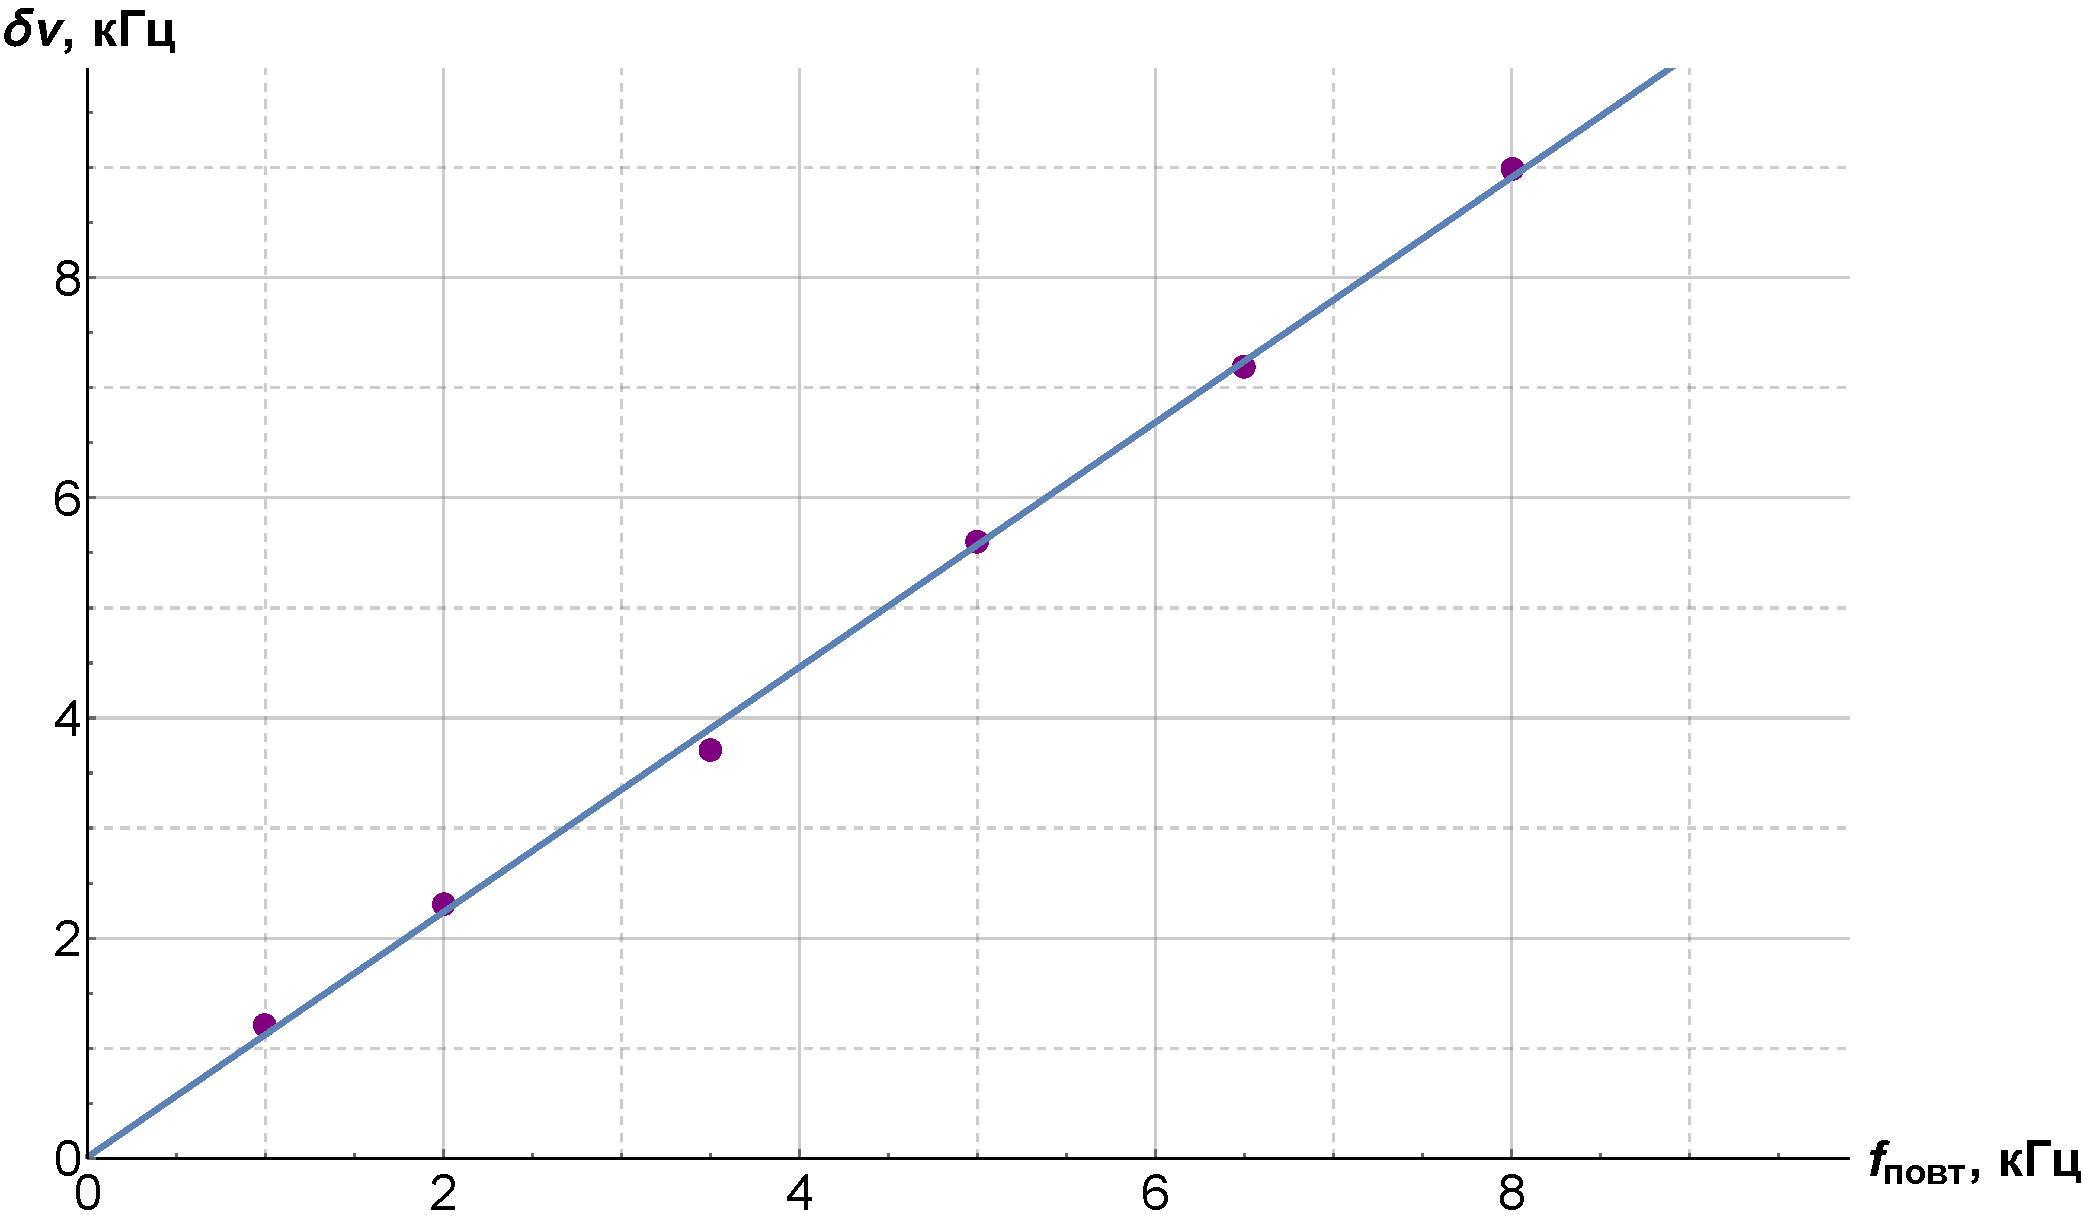
\includegraphics[scale=0.47]{B.pdf}
  		\caption{График зависимости расстояния между компонентами спектра $ \delta \nu $ от частоты повторения импульсов $ f_{повт} $}. 
  	\end{figure}
  	
  	\begin{table}[h!]
  		\centering
  		\caption{Расчет апроксимированной прямой $ y = ax +b $}
  		\begin{tabular}{c|cc}
  			\text{} & \text{Estimate} & \text{Standard Error} \\
  			\hline
  			a & 1.10 & 0.02  \\
  			b & 0.01 & 0.10  \\
  		\end{tabular}
  	\end{table}
  
  Из графика видно, что при стремлении частоты повторения к нулю стремится к нулю и расстояние между компонентами спектра.  
  
  \subsection{Исследование спектра гармонических сигналов, модулированных по амплитуде}
  	
  	Соберем схему, изображённую на рис. \ref{C}
  	Изменяя глубину модуляции на Г6-34, исследуем зависимость
  	отношения амплитуды боковой линии спектра к амплитуде основной линии $ \left(  \dfrac{A_{осн}}{А_{бок}}  \right ) $ от глубины модуляции $ m $, которая находится из отношения амплитуд на осциллографе по формуле \eqref{m}. Результаты занесем в таблицу \ref{C_table} и построим график рис. 18. 
  	
  	
  	\begin{table}[h]
  		\caption{Зависимость отношения амплитуд спектра от глубины модуляции}
  		\begin{center}
  			\begin{tabular}{|c|c|c|c|c|c|c|}
  				\hline
  				$ N $  & $ А_{min} $ & $ A_{max} $ & $ A_{осн} $ & $ A_{бок} $ & $ m $ & $ \dfrac{A_{бок}}{A_{осн}} $\\
  				\hline
  			1 & 1.0 & 1.8 & 6.0 & 1.1 & 0.29 & 0.18 \\
  			2 & 0.6 & 2.0 & 6.3 & 2.0 & 0.54 & 0.32 \\
  			3 & 0.4 & 2.3 & 6.5 & 2.7 & 0.70 & 0.42 \\
  			4 & 0.2 & 2.5 & 6.3 & 3.2 & 0.85 & 0.51 \\
  			5 & 0.8 & 1.8 & 6.3 & 1.5 & 0.38 & 0.24 \\
  				\hline
  			\end{tabular}
  		\end{center}
  		\label{C_table}
  	\end{table}
  	
  	\begin{figure}[h!]
  		\label{C_g}
  		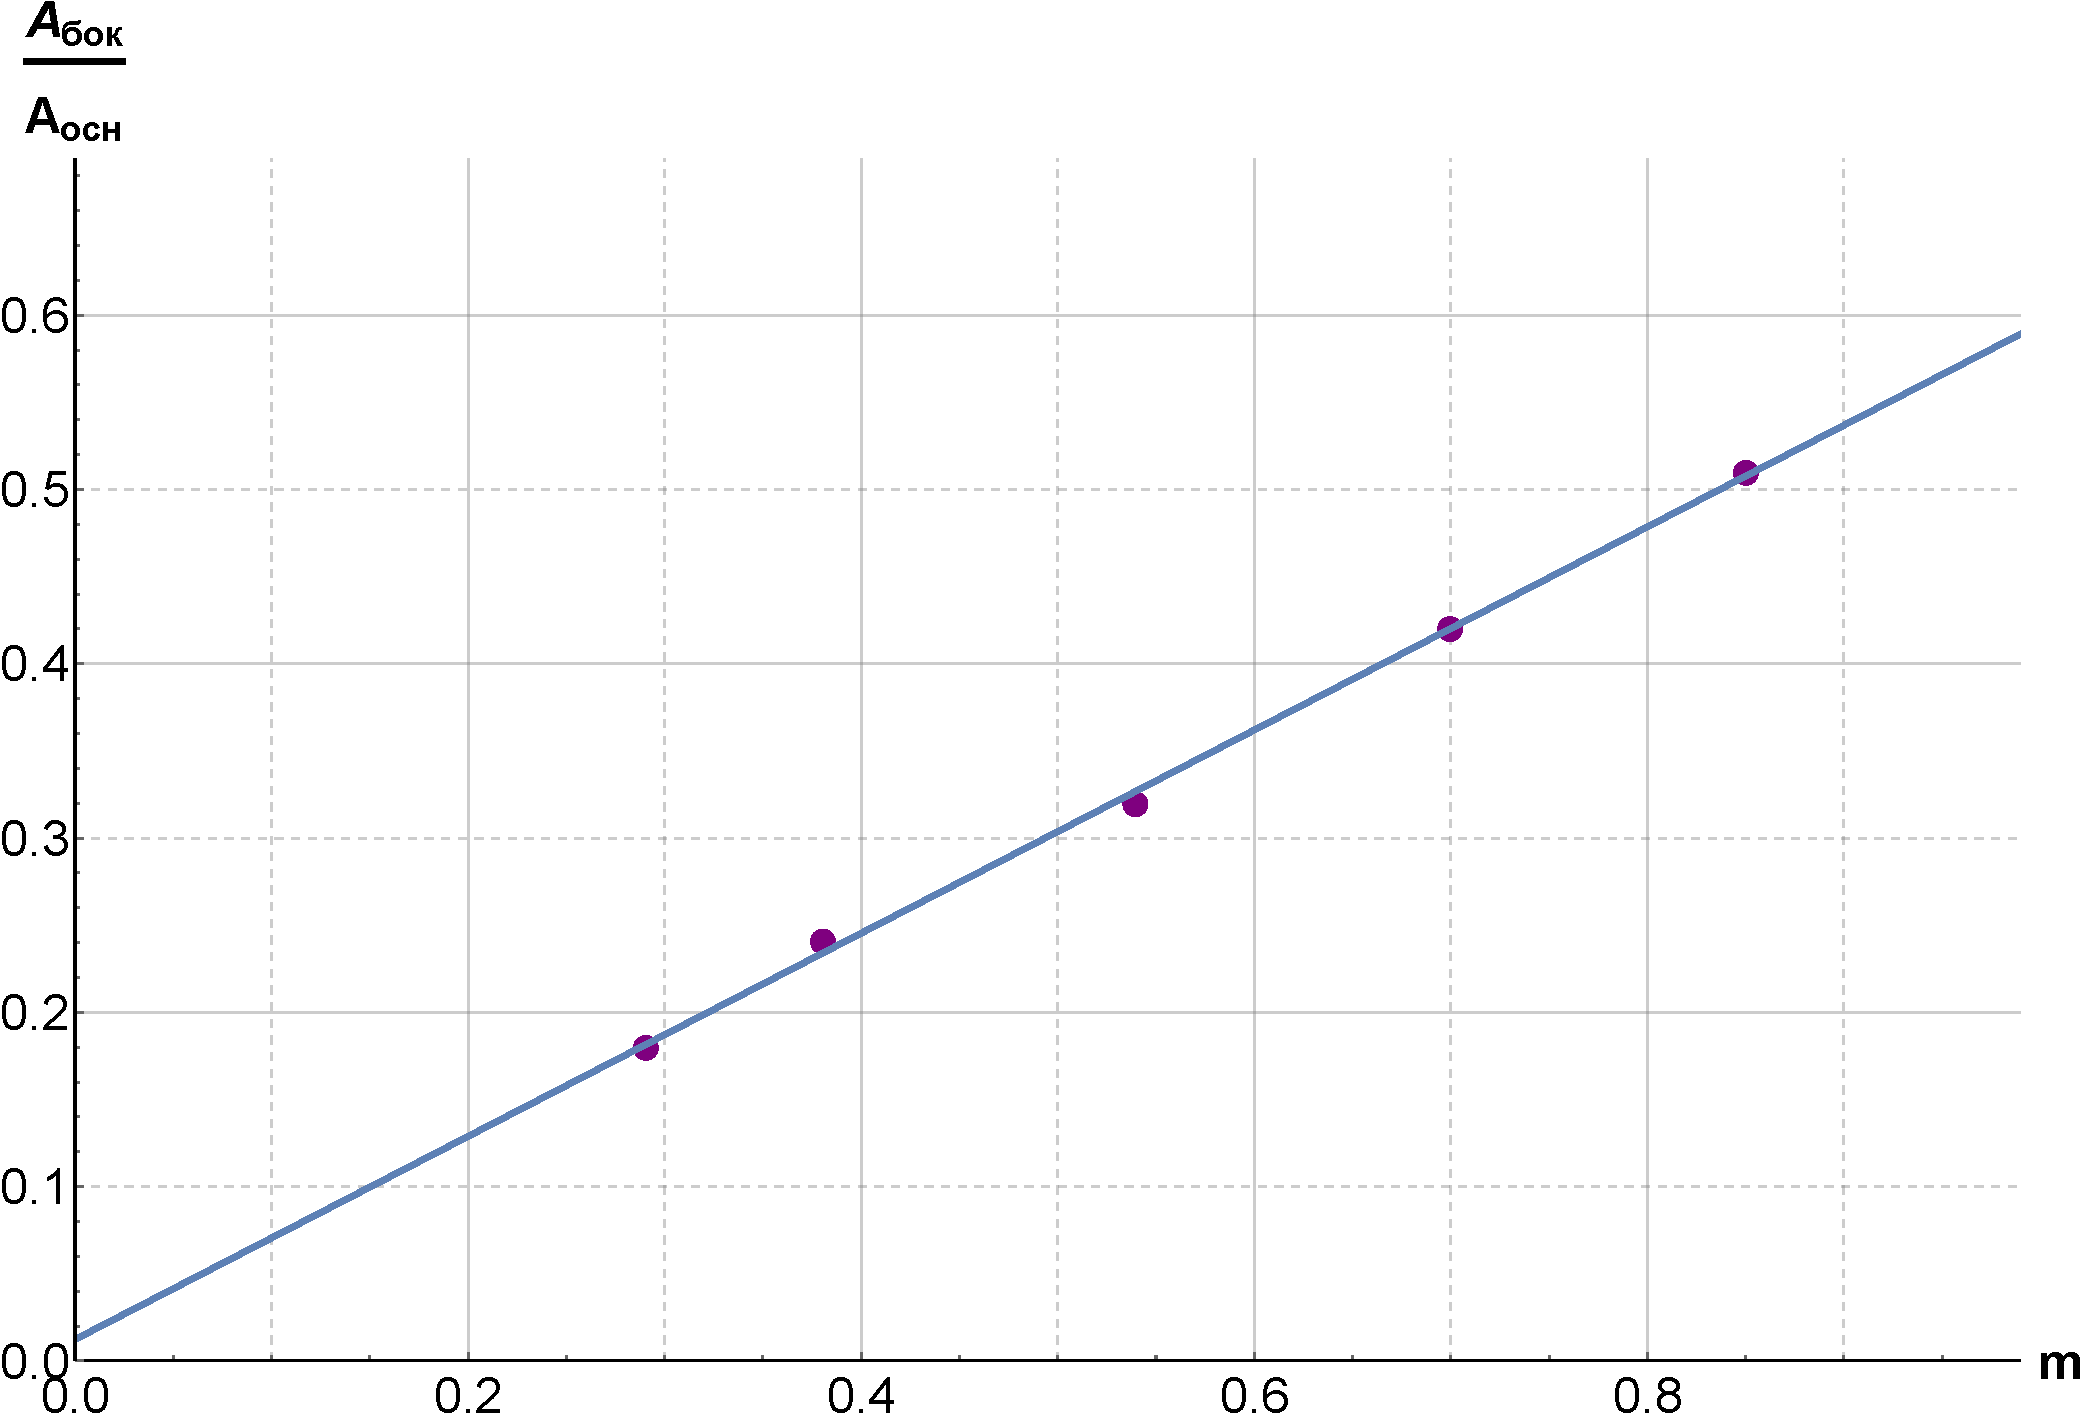
\includegraphics[scale=0.47]{C.pdf}
  		\caption{График зависимость отношения амплитуды боковой линии спектра к амплитуде основной линии $ \left(  \dfrac{A_{осн}}{А_{бок}}  \right ) $ от глубины модуляции $ m $}. 
  	\end{figure}
  	
  	\begin{table}[h!]
  		\centering
  		\caption{Расчет апроксимированной прямой $ y = ax +b $}
  		\begin{tabular}{c|cc}
  			\text{} & \text{Estimate} & \text{Standard Error} \\
  			\hline
  			a & 0.54 & 0.03 \\
  			b & 0.012 & 0.007  \\
  		\end{tabular}
  	\end{table}
  	
  	Получаем, что наш коэффициент наклона равен
  	
  	\begin{equation}\label{}
  	 a = 0,54 \pm 0,03 
  	\end{equation}
  	
  	 что примерно совпадает с теоретическим значением из формулы \eqref{a}. 
  	
  	\section{Вывод}
  	
  	В данной работе мы изучили понятие спектра и спектрального анализа, а также исследовали спектральный состав периодических электрических сигналов. 
  	
  	А именно, мы посмотрели на прямоугольные импульсы, цуги гармонических колебаний, а также гармонические сигналы, модулированные по амплитуде. Кроме того, нами был экспериментально проверен частный случай выполнения соотношения неопределённости. 
  	
  	
  	
  	
  	
  	
  	

\end{document}